\documentclass[twoside]{book}

% Packages required by doxygen
\usepackage{fixltx2e}
\usepackage{calc}
\usepackage{doxygen}
\usepackage[export]{adjustbox} % also loads graphicx
\usepackage{graphicx}
\usepackage[utf8]{inputenc}
\usepackage{makeidx}
\usepackage{multicol}
\usepackage{multirow}
\PassOptionsToPackage{warn}{textcomp}
\usepackage{textcomp}
\usepackage[nointegrals]{wasysym}
\usepackage[table]{xcolor}

% Font selection
\usepackage[T1]{fontenc}
\usepackage[scaled=.90]{helvet}
\usepackage{courier}
\usepackage{amssymb}
\usepackage{sectsty}
\renewcommand{\familydefault}{\sfdefault}
\allsectionsfont{%
  \fontseries{bc}\selectfont%
  \color{darkgray}%
}
\renewcommand{\DoxyLabelFont}{%
  \fontseries{bc}\selectfont%
  \color{darkgray}%
}
\newcommand{\+}{\discretionary{\mbox{\scriptsize$\hookleftarrow$}}{}{}}

% Page & text layout
\usepackage{geometry}
\geometry{%
  a4paper,%
  top=2.5cm,%
  bottom=2.5cm,%
  left=2.5cm,%
  right=2.5cm%
}
\tolerance=750
\hfuzz=15pt
\hbadness=750
\setlength{\emergencystretch}{15pt}
\setlength{\parindent}{0cm}
\setlength{\parskip}{3ex plus 2ex minus 2ex}
\makeatletter
\renewcommand{\paragraph}{%
  \@startsection{paragraph}{4}{0ex}{-1.0ex}{1.0ex}{%
    \normalfont\normalsize\bfseries\SS@parafont%
  }%
}
\renewcommand{\subparagraph}{%
  \@startsection{subparagraph}{5}{0ex}{-1.0ex}{1.0ex}{%
    \normalfont\normalsize\bfseries\SS@subparafont%
  }%
}
\makeatother

% Headers & footers
\usepackage{fancyhdr}
\pagestyle{fancyplain}
\fancyhead[LE]{\fancyplain{}{\bfseries\thepage}}
\fancyhead[CE]{\fancyplain{}{}}
\fancyhead[RE]{\fancyplain{}{\bfseries\leftmark}}
\fancyhead[LO]{\fancyplain{}{\bfseries\rightmark}}
\fancyhead[CO]{\fancyplain{}{}}
\fancyhead[RO]{\fancyplain{}{\bfseries\thepage}}
\fancyfoot[LE]{\fancyplain{}{}}
\fancyfoot[CE]{\fancyplain{}{}}
\fancyfoot[RE]{\fancyplain{}{\bfseries\scriptsize Generated by Doxygen }}
\fancyfoot[LO]{\fancyplain{}{\bfseries\scriptsize Generated by Doxygen }}
\fancyfoot[CO]{\fancyplain{}{}}
\fancyfoot[RO]{\fancyplain{}{}}
\renewcommand{\footrulewidth}{0.4pt}
\renewcommand{\chaptermark}[1]{%
  \markboth{#1}{}%
}
\renewcommand{\sectionmark}[1]{%
  \markright{\thesection\ #1}%
}

% Indices & bibliography
\usepackage{natbib}
\usepackage[titles]{tocloft}
\setcounter{tocdepth}{3}
\setcounter{secnumdepth}{5}
\makeindex

% Hyperlinks (required, but should be loaded last)
\usepackage{ifpdf}
\ifpdf
  \usepackage[pdftex,pagebackref=true]{hyperref}
\else
  \usepackage[ps2pdf,pagebackref=true]{hyperref}
\fi
\hypersetup{%
  colorlinks=true,%
  linkcolor=blue,%
  citecolor=blue,%
  unicode%
}

% Custom commands
\newcommand{\clearemptydoublepage}{%
  \newpage{\pagestyle{empty}\cleardoublepage}%
}

\usepackage{caption}
\captionsetup{labelsep=space,justification=centering,font={bf},singlelinecheck=off,skip=4pt,position=top}

%===== C O N T E N T S =====

\begin{document}

% Titlepage & ToC
\hypersetup{pageanchor=false,
             bookmarksnumbered=true,
             pdfencoding=unicode
            }
\pagenumbering{alph}
\begin{titlepage}
\vspace*{7cm}
\begin{center}%
{\Large Zip\+Zop }\\
\vspace*{1cm}
{\large Generated by Doxygen 1.8.13}\\
\end{center}
\end{titlepage}
\clearemptydoublepage
\pagenumbering{roman}
\tableofcontents
\clearemptydoublepage
\pagenumbering{arabic}
\hypersetup{pageanchor=true}

%--- Begin generated contents ---
\chapter{Data Structure Index}
\section{Data Structures}
Here are the data structures with brief descriptions\+:\begin{DoxyCompactList}
\item\contentsline{section}{\hyperlink{structclient}{client} \\*Struct representing a connect client in the server }{\pageref{structclient}}{}
\item\contentsline{section}{\hyperlink{structmessage}{message} \\*Struct representing a messege sent by some sender }{\pageref{structmessage}}{}
\item\contentsline{section}{\hyperlink{structsllist}{sllist} \\*A struct representing node in a singly linked list }{\pageref{structsllist}}{}
\end{DoxyCompactList}

\chapter{File Index}
\section{File List}
Here is a list of all files with brief descriptions\+:\begin{DoxyCompactList}
\item\contentsline{section}{src/\hyperlink{client_8c}{client.\+c} }{\pageref{client_8c}}{}
\item\contentsline{section}{src/\hyperlink{client_8h}{client.\+h} }{\pageref{client_8h}}{}
\item\contentsline{section}{src/\hyperlink{errcodes_8h}{errcodes.\+h} }{\pageref{errcodes_8h}}{}
\item\contentsline{section}{src/\hyperlink{message_8c}{message.\+c} }{\pageref{message_8c}}{}
\item\contentsline{section}{src/\hyperlink{message_8h}{message.\+h} }{\pageref{message_8h}}{}
\item\contentsline{section}{src/\hyperlink{sllist_8c}{sllist.\+c} }{\pageref{sllist_8c}}{}
\item\contentsline{section}{src/\hyperlink{sllist_8h}{sllist.\+h} }{\pageref{sllist_8h}}{}
\item\contentsline{section}{src/\hyperlink{zip-zop-client_8c}{zip-\/zop-\/client.\+c} }{\pageref{zip-zop-client_8c}}{}
\item\contentsline{section}{src/\hyperlink{zip-zop-server_8c}{zip-\/zop-\/server.\+c} }{\pageref{zip-zop-server_8c}}{}
\end{DoxyCompactList}

\chapter{Data Structure Documentation}
\hypertarget{structclient}{}\section{client Struct Reference}
\label{structclient}\index{client@{client}}


Struct representing a connect client in the server.  


\subsection*{Data Fields}
\begin{DoxyCompactItemize}
\item 
const char $\ast$ \hyperlink{structclient_a99f435ea140a038c3be5e2ab49aa43aa}{name}
\item 
int \hyperlink{structclient_ab7c05dd7a1a5daa5383849d8b3b0ce3f}{sockfd}
\item 
pthread\+\_\+t \hyperlink{structclient_a529fa20e309347262616a00ad0ad3d93}{thread}
\end{DoxyCompactItemize}


\subsection{Detailed Description}
Struct representing a connect client in the server. 

\subsection{Field Documentation}
\mbox{\Hypertarget{structclient_a99f435ea140a038c3be5e2ab49aa43aa}\label{structclient_a99f435ea140a038c3be5e2ab49aa43aa}} 
\index{client@{client}!name@{name}}
\index{name@{name}!client@{client}}
\subsubsection{\texorpdfstring{name}{name}}
{\footnotesize\ttfamily const char$\ast$ client\+::name}

Client name \mbox{\Hypertarget{structclient_ab7c05dd7a1a5daa5383849d8b3b0ce3f}\label{structclient_ab7c05dd7a1a5daa5383849d8b3b0ce3f}} 
\index{client@{client}!sockfd@{sockfd}}
\index{sockfd@{sockfd}!client@{client}}
\subsubsection{\texorpdfstring{sockfd}{sockfd}}
{\footnotesize\ttfamily int client\+::sockfd}

Socket that holds the connection with this client \mbox{\Hypertarget{structclient_a529fa20e309347262616a00ad0ad3d93}\label{structclient_a529fa20e309347262616a00ad0ad3d93}} 
\index{client@{client}!thread@{thread}}
\index{thread@{thread}!client@{client}}
\subsubsection{\texorpdfstring{thread}{thread}}
{\footnotesize\ttfamily pthread\+\_\+t client\+::thread}

The server thread responsible to listen to this client\textquotesingle{}s messages 

The documentation for this struct was generated from the following file\+:\begin{DoxyCompactItemize}
\item 
src/client.\+c\end{DoxyCompactItemize}

\hypertarget{structmessage}{}\section{message Struct Reference}
\label{structmessage}\index{message@{message}}


Struct representing a messege sent by some sender.  


\subsection*{Data Fields}
\begin{DoxyCompactItemize}
\item 
const char $\ast$ \hyperlink{structmessage_ad3b965525fe62cb25162084d97a3f0ff}{content}
\item 
const char $\ast$ \hyperlink{structmessage_a93d4525b657c15744e45ca9504840000}{sender\+\_\+name}
\end{DoxyCompactItemize}


\subsection{Detailed Description}
Struct representing a messege sent by some sender. 

\subsection{Field Documentation}
\mbox{\Hypertarget{structmessage_ad3b965525fe62cb25162084d97a3f0ff}\label{structmessage_ad3b965525fe62cb25162084d97a3f0ff}} 
\index{message@{message}!content@{content}}
\index{content@{content}!message@{message}}
\subsubsection{\texorpdfstring{content}{content}}
{\footnotesize\ttfamily const char$\ast$ message\+::content}

The content of the message \mbox{\Hypertarget{structmessage_a93d4525b657c15744e45ca9504840000}\label{structmessage_a93d4525b657c15744e45ca9504840000}} 
\index{message@{message}!sender\+\_\+name@{sender\+\_\+name}}
\index{sender\+\_\+name@{sender\+\_\+name}!message@{message}}
\subsubsection{\texorpdfstring{sender\+\_\+name}{sender\_name}}
{\footnotesize\ttfamily const char$\ast$ message\+::sender\+\_\+name}

The username of the sender 

The documentation for this struct was generated from the following file\+:\begin{DoxyCompactItemize}
\item 
src/\hyperlink{message_8c}{message.\+c}\end{DoxyCompactItemize}

\hypertarget{structsllist}{}\section{sllist Struct Reference}
\label{structsllist}\index{sllist@{sllist}}


Collaboration diagram for sllist\+:\nopagebreak
\begin{figure}[H]
\begin{center}
\leavevmode
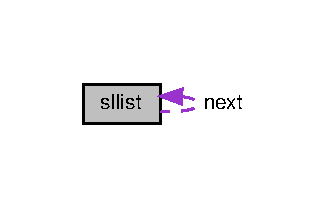
\includegraphics[width=157pt]{structsllist__coll__graph}
\end{center}
\end{figure}
\subsection*{Data Fields}
\begin{DoxyCompactItemize}
\item 
void $\ast$ \hyperlink{structsllist_aba6ff88336afdd0d2a8cb0ce396f79b6}{key}
\item 
struct \hyperlink{structsllist}{sllist} $\ast$ \hyperlink{structsllist_abd84069b1b074a7ac7d94b65672d4fd3}{next}
\end{DoxyCompactItemize}


\subsection{Field Documentation}
\mbox{\Hypertarget{structsllist_aba6ff88336afdd0d2a8cb0ce396f79b6}\label{structsllist_aba6ff88336afdd0d2a8cb0ce396f79b6}} 
\index{sllist@{sllist}!key@{key}}
\index{key@{key}!sllist@{sllist}}
\subsubsection{\texorpdfstring{key}{key}}
{\footnotesize\ttfamily void$\ast$ sllist\+::key}

\mbox{\Hypertarget{structsllist_abd84069b1b074a7ac7d94b65672d4fd3}\label{structsllist_abd84069b1b074a7ac7d94b65672d4fd3}} 
\index{sllist@{sllist}!next@{next}}
\index{next@{next}!sllist@{sllist}}
\subsubsection{\texorpdfstring{next}{next}}
{\footnotesize\ttfamily struct \hyperlink{structsllist}{sllist}$\ast$ sllist\+::next}



The documentation for this struct was generated from the following file\+:\begin{DoxyCompactItemize}
\item 
src/\hyperlink{sllist_8c}{sllist.\+c}\end{DoxyCompactItemize}

\chapter{File Documentation}
\hypertarget{client_8c}{}\section{src/client.c File Reference}
\label{client_8c}\index{src/client.\+c@{src/client.\+c}}
{\ttfamily \#include \char`\"{}client.\+h\char`\"{}}\newline
Include dependency graph for client.\+c\+:
\nopagebreak
\begin{figure}[H]
\begin{center}
\leavevmode
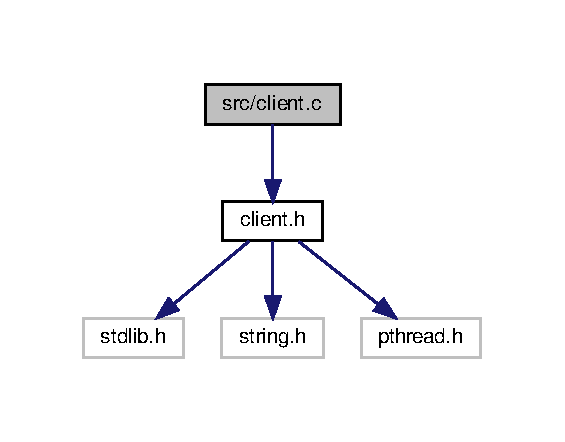
\includegraphics[width=271pt]{client_8c__incl}
\end{center}
\end{figure}
\subsection*{Data Structures}
\begin{DoxyCompactItemize}
\item 
struct \hyperlink{structclient}{client}
\end{DoxyCompactItemize}
\subsection*{Functions}
\begin{DoxyCompactItemize}
\item 
struct \hyperlink{structclient}{client} $\ast$ \hyperlink{client_8c_a2a4a2cc446bcd65f49daf665868ede23}{client\+\_\+create} (const char $\ast$name, int sockfd)
\item 
void \hyperlink{client_8c_a992d912c8130441b3a85079ab28832e9}{client\+\_\+destroy} (struct \hyperlink{structclient}{client} $\ast$c)
\item 
const char $\ast$ \hyperlink{client_8c_a609e1a23ff124b38eebeaf968f3296f3}{client\+\_\+get\+\_\+name} (struct \hyperlink{structclient}{client} $\ast$c)
\item 
int \hyperlink{client_8c_a9d2dab7f0e59959392e6b674d45a0183}{client\+\_\+get\+\_\+socket} (struct \hyperlink{structclient}{client} $\ast$c)
\item 
pthread\+\_\+t $\ast$ \hyperlink{client_8c_acbc30fcef0ca5de9f1768ff03a3af727}{client\+\_\+get\+\_\+thread} (struct \hyperlink{structclient}{client} $\ast$c)
\item 
void \hyperlink{client_8c_a1a0a4dc1973ebe7e14fb34546f870829}{client\+\_\+set\+\_\+name} (struct \hyperlink{structclient}{client} $\ast$c, const char $\ast$name)
\item 
void \hyperlink{client_8c_af6bd0240b4fb0e0128cb9d91da55f2b8}{client\+\_\+set\+\_\+socket} (struct \hyperlink{structclient}{client} $\ast$c, int sockfd)
\item 
void \hyperlink{client_8c_a8316dd83e8f2d0fff9b3953897db8f4b}{client\+\_\+set\+\_\+thread} (struct \hyperlink{structclient}{client} $\ast$c, pthread\+\_\+t thread)
\end{DoxyCompactItemize}


\subsection{Function Documentation}
\mbox{\Hypertarget{client_8c_a2a4a2cc446bcd65f49daf665868ede23}\label{client_8c_a2a4a2cc446bcd65f49daf665868ede23}} 
\index{client.\+c@{client.\+c}!client\+\_\+create@{client\+\_\+create}}
\index{client\+\_\+create@{client\+\_\+create}!client.\+c@{client.\+c}}
\subsubsection{\texorpdfstring{client\+\_\+create()}{client\_create()}}
{\footnotesize\ttfamily struct \hyperlink{structclient}{client}$\ast$ client\+\_\+create (\begin{DoxyParamCaption}\item[{const char $\ast$}]{name,  }\item[{int}]{sockfd }\end{DoxyParamCaption})}

\mbox{\Hypertarget{client_8c_a992d912c8130441b3a85079ab28832e9}\label{client_8c_a992d912c8130441b3a85079ab28832e9}} 
\index{client.\+c@{client.\+c}!client\+\_\+destroy@{client\+\_\+destroy}}
\index{client\+\_\+destroy@{client\+\_\+destroy}!client.\+c@{client.\+c}}
\subsubsection{\texorpdfstring{client\+\_\+destroy()}{client\_destroy()}}
{\footnotesize\ttfamily void client\+\_\+destroy (\begin{DoxyParamCaption}\item[{struct \hyperlink{structclient}{client} $\ast$}]{c }\end{DoxyParamCaption})}

\mbox{\Hypertarget{client_8c_a609e1a23ff124b38eebeaf968f3296f3}\label{client_8c_a609e1a23ff124b38eebeaf968f3296f3}} 
\index{client.\+c@{client.\+c}!client\+\_\+get\+\_\+name@{client\+\_\+get\+\_\+name}}
\index{client\+\_\+get\+\_\+name@{client\+\_\+get\+\_\+name}!client.\+c@{client.\+c}}
\subsubsection{\texorpdfstring{client\+\_\+get\+\_\+name()}{client\_get\_name()}}
{\footnotesize\ttfamily const char$\ast$ client\+\_\+get\+\_\+name (\begin{DoxyParamCaption}\item[{struct \hyperlink{structclient}{client} $\ast$}]{c }\end{DoxyParamCaption})}

\mbox{\Hypertarget{client_8c_a9d2dab7f0e59959392e6b674d45a0183}\label{client_8c_a9d2dab7f0e59959392e6b674d45a0183}} 
\index{client.\+c@{client.\+c}!client\+\_\+get\+\_\+socket@{client\+\_\+get\+\_\+socket}}
\index{client\+\_\+get\+\_\+socket@{client\+\_\+get\+\_\+socket}!client.\+c@{client.\+c}}
\subsubsection{\texorpdfstring{client\+\_\+get\+\_\+socket()}{client\_get\_socket()}}
{\footnotesize\ttfamily int client\+\_\+get\+\_\+socket (\begin{DoxyParamCaption}\item[{struct \hyperlink{structclient}{client} $\ast$}]{c }\end{DoxyParamCaption})}

\mbox{\Hypertarget{client_8c_acbc30fcef0ca5de9f1768ff03a3af727}\label{client_8c_acbc30fcef0ca5de9f1768ff03a3af727}} 
\index{client.\+c@{client.\+c}!client\+\_\+get\+\_\+thread@{client\+\_\+get\+\_\+thread}}
\index{client\+\_\+get\+\_\+thread@{client\+\_\+get\+\_\+thread}!client.\+c@{client.\+c}}
\subsubsection{\texorpdfstring{client\+\_\+get\+\_\+thread()}{client\_get\_thread()}}
{\footnotesize\ttfamily pthread\+\_\+t$\ast$ client\+\_\+get\+\_\+thread (\begin{DoxyParamCaption}\item[{struct \hyperlink{structclient}{client} $\ast$}]{c }\end{DoxyParamCaption})}

\mbox{\Hypertarget{client_8c_a1a0a4dc1973ebe7e14fb34546f870829}\label{client_8c_a1a0a4dc1973ebe7e14fb34546f870829}} 
\index{client.\+c@{client.\+c}!client\+\_\+set\+\_\+name@{client\+\_\+set\+\_\+name}}
\index{client\+\_\+set\+\_\+name@{client\+\_\+set\+\_\+name}!client.\+c@{client.\+c}}
\subsubsection{\texorpdfstring{client\+\_\+set\+\_\+name()}{client\_set\_name()}}
{\footnotesize\ttfamily void client\+\_\+set\+\_\+name (\begin{DoxyParamCaption}\item[{struct \hyperlink{structclient}{client} $\ast$}]{c,  }\item[{const char $\ast$}]{name }\end{DoxyParamCaption})}

\mbox{\Hypertarget{client_8c_af6bd0240b4fb0e0128cb9d91da55f2b8}\label{client_8c_af6bd0240b4fb0e0128cb9d91da55f2b8}} 
\index{client.\+c@{client.\+c}!client\+\_\+set\+\_\+socket@{client\+\_\+set\+\_\+socket}}
\index{client\+\_\+set\+\_\+socket@{client\+\_\+set\+\_\+socket}!client.\+c@{client.\+c}}
\subsubsection{\texorpdfstring{client\+\_\+set\+\_\+socket()}{client\_set\_socket()}}
{\footnotesize\ttfamily void client\+\_\+set\+\_\+socket (\begin{DoxyParamCaption}\item[{struct \hyperlink{structclient}{client} $\ast$}]{c,  }\item[{int}]{sockfd }\end{DoxyParamCaption})}

\mbox{\Hypertarget{client_8c_a8316dd83e8f2d0fff9b3953897db8f4b}\label{client_8c_a8316dd83e8f2d0fff9b3953897db8f4b}} 
\index{client.\+c@{client.\+c}!client\+\_\+set\+\_\+thread@{client\+\_\+set\+\_\+thread}}
\index{client\+\_\+set\+\_\+thread@{client\+\_\+set\+\_\+thread}!client.\+c@{client.\+c}}
\subsubsection{\texorpdfstring{client\+\_\+set\+\_\+thread()}{client\_set\_thread()}}
{\footnotesize\ttfamily void client\+\_\+set\+\_\+thread (\begin{DoxyParamCaption}\item[{struct \hyperlink{structclient}{client} $\ast$}]{c,  }\item[{pthread\+\_\+t}]{thread }\end{DoxyParamCaption})}


\hypertarget{client_8h}{}\section{src/client.h File Reference}
\label{client_8h}\index{src/client.\+h@{src/client.\+h}}
{\ttfamily \#include $<$stdlib.\+h$>$}\newline
{\ttfamily \#include $<$string.\+h$>$}\newline
{\ttfamily \#include $<$pthread.\+h$>$}\newline
Include dependency graph for client.\+h\+:\nopagebreak
\begin{figure}[H]
\begin{center}
\leavevmode
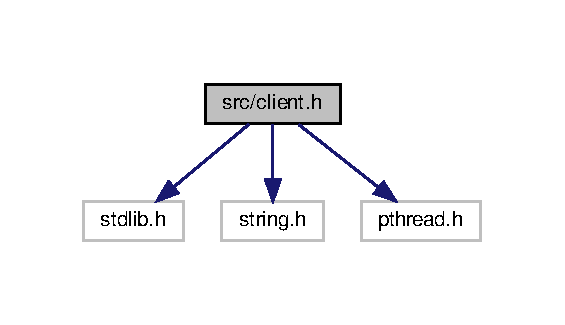
\includegraphics[width=271pt]{client_8h__incl}
\end{center}
\end{figure}
This graph shows which files directly or indirectly include this file\+:\nopagebreak
\begin{figure}[H]
\begin{center}
\leavevmode
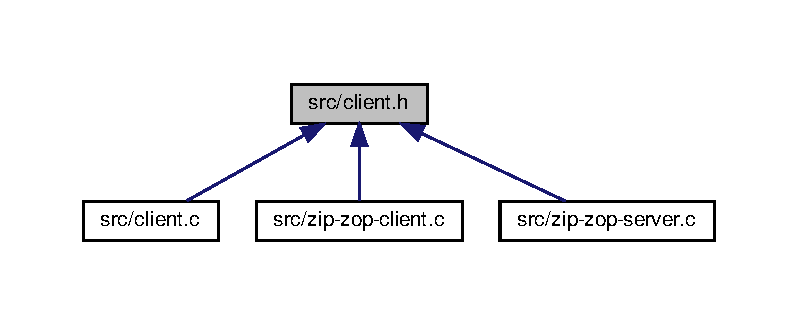
\includegraphics[width=350pt]{client_8h__dep__incl}
\end{center}
\end{figure}
\subsection*{Functions}
\begin{DoxyCompactItemize}
\item 
struct \hyperlink{structclient}{client} $\ast$ \hyperlink{client_8h_a2a4a2cc446bcd65f49daf665868ede23}{client\+\_\+create} (const char $\ast$name, int sockfd)
\begin{DoxyCompactList}\small\item\em Create a client instance. \end{DoxyCompactList}\item 
void \hyperlink{client_8h_a992d912c8130441b3a85079ab28832e9}{client\+\_\+destroy} (struct \hyperlink{structclient}{client} $\ast$c)
\item 
const char $\ast$ \hyperlink{client_8h_a609e1a23ff124b38eebeaf968f3296f3}{client\+\_\+get\+\_\+name} (struct \hyperlink{structclient}{client} $\ast$c)
\begin{DoxyCompactList}\small\item\em Get the client name. \end{DoxyCompactList}\item 
int \hyperlink{client_8h_a9d2dab7f0e59959392e6b674d45a0183}{client\+\_\+get\+\_\+socket} (struct \hyperlink{structclient}{client} $\ast$c)
\begin{DoxyCompactList}\small\item\em Get the client socket. \end{DoxyCompactList}\item 
pthread\+\_\+t $\ast$ \hyperlink{client_8h_acbc30fcef0ca5de9f1768ff03a3af727}{client\+\_\+get\+\_\+thread} (struct \hyperlink{structclient}{client} $\ast$c)
\begin{DoxyCompactList}\small\item\em Get the client thread. \end{DoxyCompactList}\item 
void \hyperlink{client_8h_a1a0a4dc1973ebe7e14fb34546f870829}{client\+\_\+set\+\_\+name} (struct \hyperlink{structclient}{client} $\ast$c, const char $\ast$name)
\begin{DoxyCompactList}\small\item\em Set the client name. \end{DoxyCompactList}\item 
void \hyperlink{client_8h_af6bd0240b4fb0e0128cb9d91da55f2b8}{client\+\_\+set\+\_\+socket} (struct \hyperlink{structclient}{client} $\ast$c, int sockfd)
\begin{DoxyCompactList}\small\item\em Set the client socket. \end{DoxyCompactList}\item 
void \hyperlink{client_8h_a8316dd83e8f2d0fff9b3953897db8f4b}{client\+\_\+set\+\_\+thread} (struct \hyperlink{structclient}{client} $\ast$c, pthread\+\_\+t thread)
\begin{DoxyCompactList}\small\item\em Set the client thread. \end{DoxyCompactList}\end{DoxyCompactItemize}


\subsection{Function Documentation}
\mbox{\Hypertarget{client_8h_a2a4a2cc446bcd65f49daf665868ede23}\label{client_8h_a2a4a2cc446bcd65f49daf665868ede23}} 
\index{client.\+h@{client.\+h}!client\+\_\+create@{client\+\_\+create}}
\index{client\+\_\+create@{client\+\_\+create}!client.\+h@{client.\+h}}
\subsubsection{\texorpdfstring{client\+\_\+create()}{client\_create()}}
{\footnotesize\ttfamily struct \hyperlink{structclient}{client}$\ast$ client\+\_\+create (\begin{DoxyParamCaption}\item[{const char $\ast$}]{name,  }\item[{int}]{sockfd }\end{DoxyParamCaption})}



Create a client instance. 

Both parameters will be copied into the message, so the user is free to {\ttfamily free()} the parameters passed to this function if necessary.


\begin{DoxyParams}[1]{Parameters}
\mbox{\tt in}  & {\em name} & The client name. \\
\hline
\mbox{\tt in}  & {\em sockfd} & The socket connected to this client.\\
\hline
\end{DoxyParams}
\begin{DoxyReturn}{Returns}
A pointer to the client in case of success, N\+U\+LL otherwise. The client must be freed, using \hyperlink{client_8c_a992d912c8130441b3a85079ab28832e9}{client\+\_\+destroy()}.
\end{DoxyReturn}
\begin{DoxySeeAlso}{See also}
\hyperlink{client_8c_a992d912c8130441b3a85079ab28832e9}{client\+\_\+destroy} 
\end{DoxySeeAlso}
\mbox{\Hypertarget{client_8h_a992d912c8130441b3a85079ab28832e9}\label{client_8h_a992d912c8130441b3a85079ab28832e9}} 
\index{client.\+h@{client.\+h}!client\+\_\+destroy@{client\+\_\+destroy}}
\index{client\+\_\+destroy@{client\+\_\+destroy}!client.\+h@{client.\+h}}
\subsubsection{\texorpdfstring{client\+\_\+destroy()}{client\_destroy()}}
{\footnotesize\ttfamily void client\+\_\+destroy (\begin{DoxyParamCaption}\item[{struct \hyperlink{structclient}{client} $\ast$}]{c }\end{DoxyParamCaption})}

Destroys a client.


\begin{DoxyParams}[1]{Parameters}
\mbox{\tt in}  & {\em c} & A pointer to the client. \\
\hline
\end{DoxyParams}
\mbox{\Hypertarget{client_8h_a609e1a23ff124b38eebeaf968f3296f3}\label{client_8h_a609e1a23ff124b38eebeaf968f3296f3}} 
\index{client.\+h@{client.\+h}!client\+\_\+get\+\_\+name@{client\+\_\+get\+\_\+name}}
\index{client\+\_\+get\+\_\+name@{client\+\_\+get\+\_\+name}!client.\+h@{client.\+h}}
\subsubsection{\texorpdfstring{client\+\_\+get\+\_\+name()}{client\_get\_name()}}
{\footnotesize\ttfamily const char$\ast$ client\+\_\+get\+\_\+name (\begin{DoxyParamCaption}\item[{struct \hyperlink{structclient}{client} $\ast$}]{c }\end{DoxyParamCaption})}



Get the client name. 


\begin{DoxyParams}[1]{Parameters}
\mbox{\tt in}  & {\em c} & The client.\\
\hline
\end{DoxyParams}
\begin{DoxyReturn}{Returns}
The client name. 
\end{DoxyReturn}
\mbox{\Hypertarget{client_8h_a9d2dab7f0e59959392e6b674d45a0183}\label{client_8h_a9d2dab7f0e59959392e6b674d45a0183}} 
\index{client.\+h@{client.\+h}!client\+\_\+get\+\_\+socket@{client\+\_\+get\+\_\+socket}}
\index{client\+\_\+get\+\_\+socket@{client\+\_\+get\+\_\+socket}!client.\+h@{client.\+h}}
\subsubsection{\texorpdfstring{client\+\_\+get\+\_\+socket()}{client\_get\_socket()}}
{\footnotesize\ttfamily int client\+\_\+get\+\_\+socket (\begin{DoxyParamCaption}\item[{struct \hyperlink{structclient}{client} $\ast$}]{c }\end{DoxyParamCaption})}



Get the client socket. 


\begin{DoxyParams}[1]{Parameters}
\mbox{\tt in}  & {\em c} & The client.\\
\hline
\end{DoxyParams}
\begin{DoxyReturn}{Returns}
The client socket. 
\end{DoxyReturn}
\mbox{\Hypertarget{client_8h_acbc30fcef0ca5de9f1768ff03a3af727}\label{client_8h_acbc30fcef0ca5de9f1768ff03a3af727}} 
\index{client.\+h@{client.\+h}!client\+\_\+get\+\_\+thread@{client\+\_\+get\+\_\+thread}}
\index{client\+\_\+get\+\_\+thread@{client\+\_\+get\+\_\+thread}!client.\+h@{client.\+h}}
\subsubsection{\texorpdfstring{client\+\_\+get\+\_\+thread()}{client\_get\_thread()}}
{\footnotesize\ttfamily pthread\+\_\+t$\ast$ client\+\_\+get\+\_\+thread (\begin{DoxyParamCaption}\item[{struct \hyperlink{structclient}{client} $\ast$}]{c }\end{DoxyParamCaption})}



Get the client thread. 


\begin{DoxyParams}[1]{Parameters}
\mbox{\tt in}  & {\em c} & The client.\\
\hline
\end{DoxyParams}
\begin{DoxyReturn}{Returns}
An Address of the client thread.
\end{DoxyReturn}
\begin{DoxyWarning}{Warning}
This function returns the address of the actual thread stored in the client. Do not try to free this address. 
\end{DoxyWarning}
\mbox{\Hypertarget{client_8h_a1a0a4dc1973ebe7e14fb34546f870829}\label{client_8h_a1a0a4dc1973ebe7e14fb34546f870829}} 
\index{client.\+h@{client.\+h}!client\+\_\+set\+\_\+name@{client\+\_\+set\+\_\+name}}
\index{client\+\_\+set\+\_\+name@{client\+\_\+set\+\_\+name}!client.\+h@{client.\+h}}
\subsubsection{\texorpdfstring{client\+\_\+set\+\_\+name()}{client\_set\_name()}}
{\footnotesize\ttfamily void client\+\_\+set\+\_\+name (\begin{DoxyParamCaption}\item[{struct \hyperlink{structclient}{client} $\ast$}]{c,  }\item[{const char $\ast$}]{name }\end{DoxyParamCaption})}



Set the client name. 


\begin{DoxyParams}[1]{Parameters}
\mbox{\tt in}  & {\em c} & The client. \\
\hline
\mbox{\tt in}  & {\em name} & The client name. \\
\hline
\end{DoxyParams}
\mbox{\Hypertarget{client_8h_af6bd0240b4fb0e0128cb9d91da55f2b8}\label{client_8h_af6bd0240b4fb0e0128cb9d91da55f2b8}} 
\index{client.\+h@{client.\+h}!client\+\_\+set\+\_\+socket@{client\+\_\+set\+\_\+socket}}
\index{client\+\_\+set\+\_\+socket@{client\+\_\+set\+\_\+socket}!client.\+h@{client.\+h}}
\subsubsection{\texorpdfstring{client\+\_\+set\+\_\+socket()}{client\_set\_socket()}}
{\footnotesize\ttfamily void client\+\_\+set\+\_\+socket (\begin{DoxyParamCaption}\item[{struct \hyperlink{structclient}{client} $\ast$}]{c,  }\item[{int}]{sockfd }\end{DoxyParamCaption})}



Set the client socket. 


\begin{DoxyParams}[1]{Parameters}
\mbox{\tt in}  & {\em c} & The client. \\
\hline
\mbox{\tt in}  & {\em sockfd} & The client socket. \\
\hline
\end{DoxyParams}
\mbox{\Hypertarget{client_8h_a8316dd83e8f2d0fff9b3953897db8f4b}\label{client_8h_a8316dd83e8f2d0fff9b3953897db8f4b}} 
\index{client.\+h@{client.\+h}!client\+\_\+set\+\_\+thread@{client\+\_\+set\+\_\+thread}}
\index{client\+\_\+set\+\_\+thread@{client\+\_\+set\+\_\+thread}!client.\+h@{client.\+h}}
\subsubsection{\texorpdfstring{client\+\_\+set\+\_\+thread()}{client\_set\_thread()}}
{\footnotesize\ttfamily void client\+\_\+set\+\_\+thread (\begin{DoxyParamCaption}\item[{struct \hyperlink{structclient}{client} $\ast$}]{c,  }\item[{pthread\+\_\+t}]{thread }\end{DoxyParamCaption})}



Set the client thread. 


\begin{DoxyParams}[1]{Parameters}
\mbox{\tt in}  & {\em c} & The client. \\
\hline
\mbox{\tt in}  & {\em thread} & The client thread. \\
\hline
\end{DoxyParams}

\hypertarget{errcodes_8h}{}\section{src/errcodes.h File Reference}
\label{errcodes_8h}\index{src/errcodes.\+h@{src/errcodes.\+h}}
This graph shows which files directly or indirectly include this file\+:\nopagebreak
\begin{figure}[H]
\begin{center}
\leavevmode
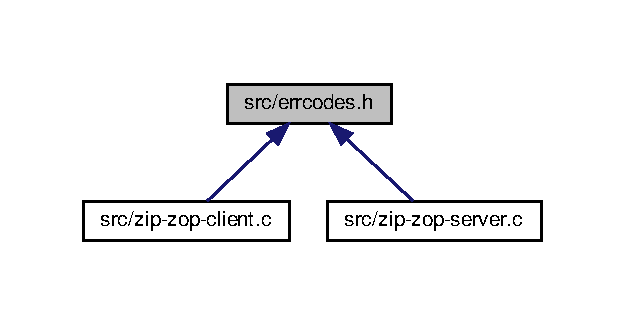
\includegraphics[width=300pt]{errcodes_8h__dep__incl}
\end{center}
\end{figure}
\subsection*{Enumerations}
\begin{DoxyCompactItemize}
\item 
enum \hyperlink{errcodes_8h_ae12919244f12ac834cf060252b251fae}{errcodes} \{ \newline
\hyperlink{errcodes_8h_ae12919244f12ac834cf060252b251faeac3121e429a129b2ccb51a92b7c78c4b4}{E\+\_\+\+S\+U\+C\+C\+E\+SS}, 
\hyperlink{errcodes_8h_ae12919244f12ac834cf060252b251faea00bc19f90f0e6d524064013b7ab4937f}{E\+\_\+\+G\+E\+T\+A\+D\+D\+R\+I\+N\+FO}, 
\hyperlink{errcodes_8h_ae12919244f12ac834cf060252b251faea040cb529b2f2572998034727de2c14f3}{E\+\_\+\+B\+I\+ND}, 
\hyperlink{errcodes_8h_ae12919244f12ac834cf060252b251faeaadf03f6fdac4cf380805d1b39975699c}{E\+\_\+\+L\+I\+S\+T\+EN}, 
\newline
\hyperlink{errcodes_8h_ae12919244f12ac834cf060252b251faeab324900900daaf0d32a6331c17919721}{E\+\_\+\+B\+A\+D\+\_\+\+A\+R\+GS}, 
\hyperlink{errcodes_8h_ae12919244f12ac834cf060252b251faeac7c517b61a6e9edb881ed9ad34d36deb}{E\+\_\+\+C\+O\+N\+N\+E\+CT}, 
\hyperlink{errcodes_8h_ae12919244f12ac834cf060252b251faeaef1d987bb49f358ed8b08170553c15b9}{E\+\_\+\+P\+T\+H\+R\+E\+A\+D\+\_\+\+C\+R\+E\+A\+TE}
 \}
\end{DoxyCompactItemize}


\subsection{Enumeration Type Documentation}
\mbox{\Hypertarget{errcodes_8h_ae12919244f12ac834cf060252b251fae}\label{errcodes_8h_ae12919244f12ac834cf060252b251fae}} 
\index{errcodes.\+h@{errcodes.\+h}!errcodes@{errcodes}}
\index{errcodes@{errcodes}!errcodes.\+h@{errcodes.\+h}}
\subsubsection{\texorpdfstring{errcodes}{errcodes}}
{\footnotesize\ttfamily enum \hyperlink{errcodes_8h_ae12919244f12ac834cf060252b251fae}{errcodes}}

\begin{DoxyEnumFields}{Enumerator}
\raisebox{\heightof{T}}[0pt][0pt]{\index{E\+\_\+\+S\+U\+C\+C\+E\+SS@{E\+\_\+\+S\+U\+C\+C\+E\+SS}!errcodes.\+h@{errcodes.\+h}}\index{errcodes.\+h@{errcodes.\+h}!E\+\_\+\+S\+U\+C\+C\+E\+SS@{E\+\_\+\+S\+U\+C\+C\+E\+SS}}}\mbox{\Hypertarget{errcodes_8h_ae12919244f12ac834cf060252b251faeac3121e429a129b2ccb51a92b7c78c4b4}\label{errcodes_8h_ae12919244f12ac834cf060252b251faeac3121e429a129b2ccb51a92b7c78c4b4}} 
E\+\_\+\+S\+U\+C\+C\+E\+SS&\\
\hline

\raisebox{\heightof{T}}[0pt][0pt]{\index{E\+\_\+\+G\+E\+T\+A\+D\+D\+R\+I\+N\+FO@{E\+\_\+\+G\+E\+T\+A\+D\+D\+R\+I\+N\+FO}!errcodes.\+h@{errcodes.\+h}}\index{errcodes.\+h@{errcodes.\+h}!E\+\_\+\+G\+E\+T\+A\+D\+D\+R\+I\+N\+FO@{E\+\_\+\+G\+E\+T\+A\+D\+D\+R\+I\+N\+FO}}}\mbox{\Hypertarget{errcodes_8h_ae12919244f12ac834cf060252b251faea00bc19f90f0e6d524064013b7ab4937f}\label{errcodes_8h_ae12919244f12ac834cf060252b251faea00bc19f90f0e6d524064013b7ab4937f}} 
E\+\_\+\+G\+E\+T\+A\+D\+D\+R\+I\+N\+FO&\\
\hline

\raisebox{\heightof{T}}[0pt][0pt]{\index{E\+\_\+\+B\+I\+ND@{E\+\_\+\+B\+I\+ND}!errcodes.\+h@{errcodes.\+h}}\index{errcodes.\+h@{errcodes.\+h}!E\+\_\+\+B\+I\+ND@{E\+\_\+\+B\+I\+ND}}}\mbox{\Hypertarget{errcodes_8h_ae12919244f12ac834cf060252b251faea040cb529b2f2572998034727de2c14f3}\label{errcodes_8h_ae12919244f12ac834cf060252b251faea040cb529b2f2572998034727de2c14f3}} 
E\+\_\+\+B\+I\+ND&\\
\hline

\raisebox{\heightof{T}}[0pt][0pt]{\index{E\+\_\+\+L\+I\+S\+T\+EN@{E\+\_\+\+L\+I\+S\+T\+EN}!errcodes.\+h@{errcodes.\+h}}\index{errcodes.\+h@{errcodes.\+h}!E\+\_\+\+L\+I\+S\+T\+EN@{E\+\_\+\+L\+I\+S\+T\+EN}}}\mbox{\Hypertarget{errcodes_8h_ae12919244f12ac834cf060252b251faeaadf03f6fdac4cf380805d1b39975699c}\label{errcodes_8h_ae12919244f12ac834cf060252b251faeaadf03f6fdac4cf380805d1b39975699c}} 
E\+\_\+\+L\+I\+S\+T\+EN&\\
\hline

\raisebox{\heightof{T}}[0pt][0pt]{\index{E\+\_\+\+B\+A\+D\+\_\+\+A\+R\+GS@{E\+\_\+\+B\+A\+D\+\_\+\+A\+R\+GS}!errcodes.\+h@{errcodes.\+h}}\index{errcodes.\+h@{errcodes.\+h}!E\+\_\+\+B\+A\+D\+\_\+\+A\+R\+GS@{E\+\_\+\+B\+A\+D\+\_\+\+A\+R\+GS}}}\mbox{\Hypertarget{errcodes_8h_ae12919244f12ac834cf060252b251faeab324900900daaf0d32a6331c17919721}\label{errcodes_8h_ae12919244f12ac834cf060252b251faeab324900900daaf0d32a6331c17919721}} 
E\+\_\+\+B\+A\+D\+\_\+\+A\+R\+GS&\\
\hline

\raisebox{\heightof{T}}[0pt][0pt]{\index{E\+\_\+\+C\+O\+N\+N\+E\+CT@{E\+\_\+\+C\+O\+N\+N\+E\+CT}!errcodes.\+h@{errcodes.\+h}}\index{errcodes.\+h@{errcodes.\+h}!E\+\_\+\+C\+O\+N\+N\+E\+CT@{E\+\_\+\+C\+O\+N\+N\+E\+CT}}}\mbox{\Hypertarget{errcodes_8h_ae12919244f12ac834cf060252b251faeac7c517b61a6e9edb881ed9ad34d36deb}\label{errcodes_8h_ae12919244f12ac834cf060252b251faeac7c517b61a6e9edb881ed9ad34d36deb}} 
E\+\_\+\+C\+O\+N\+N\+E\+CT&\\
\hline

\raisebox{\heightof{T}}[0pt][0pt]{\index{E\+\_\+\+P\+T\+H\+R\+E\+A\+D\+\_\+\+C\+R\+E\+A\+TE@{E\+\_\+\+P\+T\+H\+R\+E\+A\+D\+\_\+\+C\+R\+E\+A\+TE}!errcodes.\+h@{errcodes.\+h}}\index{errcodes.\+h@{errcodes.\+h}!E\+\_\+\+P\+T\+H\+R\+E\+A\+D\+\_\+\+C\+R\+E\+A\+TE@{E\+\_\+\+P\+T\+H\+R\+E\+A\+D\+\_\+\+C\+R\+E\+A\+TE}}}\mbox{\Hypertarget{errcodes_8h_ae12919244f12ac834cf060252b251faeaef1d987bb49f358ed8b08170553c15b9}\label{errcodes_8h_ae12919244f12ac834cf060252b251faeaef1d987bb49f358ed8b08170553c15b9}} 
E\+\_\+\+P\+T\+H\+R\+E\+A\+D\+\_\+\+C\+R\+E\+A\+TE&\\
\hline

\end{DoxyEnumFields}

\hypertarget{message_8c}{}\section{src/message.c File Reference}
\label{message_8c}\index{src/message.\+c@{src/message.\+c}}
{\ttfamily \#include \char`\"{}message.\+h\char`\"{}}\newline
Include dependency graph for message.\+c\+:\nopagebreak
\begin{figure}[H]
\begin{center}
\leavevmode
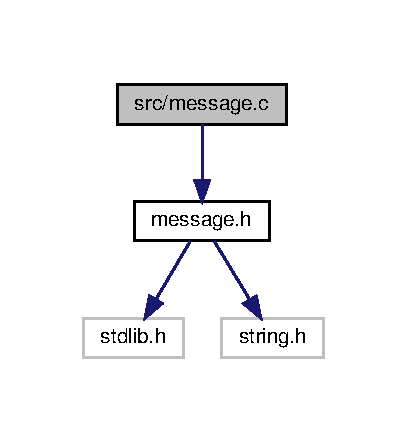
\includegraphics[width=196pt]{message_8c__incl}
\end{center}
\end{figure}
\subsection*{Data Structures}
\begin{DoxyCompactItemize}
\item 
struct \hyperlink{structmessage}{message}
\begin{DoxyCompactList}\small\item\em Struct representing a messege sent by some sender. \end{DoxyCompactList}\end{DoxyCompactItemize}
\subsection*{Functions}
\begin{DoxyCompactItemize}
\item 
struct \hyperlink{structmessage}{message} $\ast$ \hyperlink{message_8c_af0270eefb03058e936215fd11fde4b93}{message\+\_\+create} (const char $\ast$content, const char $\ast$sender\+\_\+name)
\begin{DoxyCompactList}\small\item\em Creates a message. \end{DoxyCompactList}\item 
void \hyperlink{message_8c_ad0eaa8623d0f22248ec230fd91bd819b}{message\+\_\+destroy} (struct \hyperlink{structmessage}{message} $\ast$m)
\begin{DoxyCompactList}\small\item\em Destroys a message. \end{DoxyCompactList}\item 
const char $\ast$ \hyperlink{message_8c_a31cd31a7acd86c44c38238f5a5b1da76}{message\+\_\+get\+\_\+content} (struct \hyperlink{structmessage}{message} $\ast$m)
\begin{DoxyCompactList}\small\item\em Get the message content. \end{DoxyCompactList}\item 
const char $\ast$ \hyperlink{message_8c_ac6e3d955212965dc1ab7b5e3f88bc535}{message\+\_\+get\+\_\+sender} (struct \hyperlink{structmessage}{message} $\ast$m)
\begin{DoxyCompactList}\small\item\em Get the message sender. \end{DoxyCompactList}\item 
char $\ast$ \hyperlink{message_8c_a0e07715664284f7a821216ca83317e60}{message\+\_\+pack} (struct \hyperlink{structmessage}{message} $\ast$m, int $\ast$len)
\begin{DoxyCompactList}\small\item\em Serialize a message. \end{DoxyCompactList}\item 
struct \hyperlink{structmessage}{message} $\ast$ \hyperlink{message_8c_a3ba54a38dd0b04dea973f33437bb9125}{message\+\_\+unpack} (char $\ast$pack)
\begin{DoxyCompactList}\small\item\em Deserialize a message. \end{DoxyCompactList}\end{DoxyCompactItemize}


\subsection{Function Documentation}
\mbox{\Hypertarget{message_8c_af0270eefb03058e936215fd11fde4b93}\label{message_8c_af0270eefb03058e936215fd11fde4b93}} 
\index{message.\+c@{message.\+c}!message\+\_\+create@{message\+\_\+create}}
\index{message\+\_\+create@{message\+\_\+create}!message.\+c@{message.\+c}}
\subsubsection{\texorpdfstring{message\+\_\+create()}{message\_create()}}
{\footnotesize\ttfamily struct \hyperlink{structmessage}{message}$\ast$ message\+\_\+create (\begin{DoxyParamCaption}\item[{const char $\ast$}]{content,  }\item[{const char $\ast$}]{sender\+\_\+name }\end{DoxyParamCaption})}



Creates a message. 

Both parameters will be copied into the message, so the user is free to {\ttfamily free()} the parameters passed to this function if necessary.


\begin{DoxyParams}[1]{Parameters}
\mbox{\tt in}  & {\em content} & The content of the message. \\
\hline
\mbox{\tt in}  & {\em sender\+\_\+name} & The username of the sender.\\
\hline
\end{DoxyParams}
\begin{DoxyReturn}{Returns}
A pointer to a struct message in case of success, N\+U\+LL otherwise. The message must be freed, using \hyperlink{message_8c_ad0eaa8623d0f22248ec230fd91bd819b}{message\+\_\+destroy()}, when is not needed anymore. 
\end{DoxyReturn}
\begin{DoxySeeAlso}{See also}
\hyperlink{message_8c_ad0eaa8623d0f22248ec230fd91bd819b}{message\+\_\+destroy} 
\end{DoxySeeAlso}
\mbox{\Hypertarget{message_8c_ad0eaa8623d0f22248ec230fd91bd819b}\label{message_8c_ad0eaa8623d0f22248ec230fd91bd819b}} 
\index{message.\+c@{message.\+c}!message\+\_\+destroy@{message\+\_\+destroy}}
\index{message\+\_\+destroy@{message\+\_\+destroy}!message.\+c@{message.\+c}}
\subsubsection{\texorpdfstring{message\+\_\+destroy()}{message\_destroy()}}
{\footnotesize\ttfamily void message\+\_\+destroy (\begin{DoxyParamCaption}\item[{struct \hyperlink{structmessage}{message} $\ast$}]{m }\end{DoxyParamCaption})}



Destroys a message. 


\begin{DoxyParams}[1]{Parameters}
\mbox{\tt in}  & {\em m} & A pointer to the message.\\
\hline
\end{DoxyParams}
\begin{DoxySeeAlso}{See also}
\hyperlink{message_8c_af0270eefb03058e936215fd11fde4b93}{message\+\_\+create} 
\end{DoxySeeAlso}
\mbox{\Hypertarget{message_8c_a31cd31a7acd86c44c38238f5a5b1da76}\label{message_8c_a31cd31a7acd86c44c38238f5a5b1da76}} 
\index{message.\+c@{message.\+c}!message\+\_\+get\+\_\+content@{message\+\_\+get\+\_\+content}}
\index{message\+\_\+get\+\_\+content@{message\+\_\+get\+\_\+content}!message.\+c@{message.\+c}}
\subsubsection{\texorpdfstring{message\+\_\+get\+\_\+content()}{message\_get\_content()}}
{\footnotesize\ttfamily const char$\ast$ message\+\_\+get\+\_\+content (\begin{DoxyParamCaption}\item[{struct \hyperlink{structmessage}{message} $\ast$}]{m }\end{DoxyParamCaption})}



Get the message content. 


\begin{DoxyParams}[1]{Parameters}
\mbox{\tt in}  & {\em m} & A pointer to the message.\\
\hline
\end{DoxyParams}
\begin{DoxyReturn}{Returns}
A pointer to the message content.
\end{DoxyReturn}
\begin{DoxyWarning}{Warning}
The returned value should not be freed. 
\end{DoxyWarning}
\mbox{\Hypertarget{message_8c_ac6e3d955212965dc1ab7b5e3f88bc535}\label{message_8c_ac6e3d955212965dc1ab7b5e3f88bc535}} 
\index{message.\+c@{message.\+c}!message\+\_\+get\+\_\+sender@{message\+\_\+get\+\_\+sender}}
\index{message\+\_\+get\+\_\+sender@{message\+\_\+get\+\_\+sender}!message.\+c@{message.\+c}}
\subsubsection{\texorpdfstring{message\+\_\+get\+\_\+sender()}{message\_get\_sender()}}
{\footnotesize\ttfamily const char$\ast$ message\+\_\+get\+\_\+sender (\begin{DoxyParamCaption}\item[{struct \hyperlink{structmessage}{message} $\ast$}]{m }\end{DoxyParamCaption})}



Get the message sender. 


\begin{DoxyParams}[1]{Parameters}
\mbox{\tt in}  & {\em m} & A pointer to the message.\\
\hline
\end{DoxyParams}
\begin{DoxyReturn}{Returns}
A pointer to the sender name.
\end{DoxyReturn}
\begin{DoxyWarning}{Warning}
The returned value should not be freed. 
\end{DoxyWarning}
\mbox{\Hypertarget{message_8c_a0e07715664284f7a821216ca83317e60}\label{message_8c_a0e07715664284f7a821216ca83317e60}} 
\index{message.\+c@{message.\+c}!message\+\_\+pack@{message\+\_\+pack}}
\index{message\+\_\+pack@{message\+\_\+pack}!message.\+c@{message.\+c}}
\subsubsection{\texorpdfstring{message\+\_\+pack()}{message\_pack()}}
{\footnotesize\ttfamily char$\ast$ message\+\_\+pack (\begin{DoxyParamCaption}\item[{struct \hyperlink{structmessage}{message} $\ast$}]{m,  }\item[{int $\ast$}]{len }\end{DoxyParamCaption})}



Serialize a message. 

Pack/\+Serialize the struct message in a format that can be sent through the network.


\begin{DoxyParams}[1]{Parameters}
\mbox{\tt in}  & {\em m} & A pointer to the message. \\
\hline
\mbox{\tt out}  & {\em len} & A pointer to a integer where the length of the serialized message will be stored.\\
\hline
\end{DoxyParams}
\begin{DoxyReturn}{Returns}
A pointer to the serialized message. This should be freed when is not necessary anymore.
\end{DoxyReturn}
\begin{DoxySeeAlso}{See also}
\hyperlink{message_8c_a3ba54a38dd0b04dea973f33437bb9125}{message\+\_\+unpack} 
\end{DoxySeeAlso}
\mbox{\Hypertarget{message_8c_a3ba54a38dd0b04dea973f33437bb9125}\label{message_8c_a3ba54a38dd0b04dea973f33437bb9125}} 
\index{message.\+c@{message.\+c}!message\+\_\+unpack@{message\+\_\+unpack}}
\index{message\+\_\+unpack@{message\+\_\+unpack}!message.\+c@{message.\+c}}
\subsubsection{\texorpdfstring{message\+\_\+unpack()}{message\_unpack()}}
{\footnotesize\ttfamily struct \hyperlink{structmessage}{message}$\ast$ message\+\_\+unpack (\begin{DoxyParamCaption}\item[{char $\ast$}]{pack }\end{DoxyParamCaption})}



Deserialize a message. 

Unpack/\+Deserialize a string into a struct message.


\begin{DoxyParams}[1]{Parameters}
\mbox{\tt in}  & {\em pack} & The string that represent the packed message generated by \hyperlink{message_8c_a0e07715664284f7a821216ca83317e60}{message\+\_\+pack()}.\\
\hline
\end{DoxyParams}
\begin{DoxyReturn}{Returns}
A pointer to the deserialized message. This should be freed when is not necessary anymore.
\end{DoxyReturn}
\begin{DoxySeeAlso}{See also}
\hyperlink{message_8c_a0e07715664284f7a821216ca83317e60}{message\+\_\+pack} 
\end{DoxySeeAlso}

\hypertarget{message_8h}{}\section{src/message.h File Reference}
\label{message_8h}\index{src/message.\+h@{src/message.\+h}}
{\ttfamily \#include $<$stdlib.\+h$>$}\newline
{\ttfamily \#include $<$string.\+h$>$}\newline
Include dependency graph for message.\+h\+:\nopagebreak
\begin{figure}[H]
\begin{center}
\leavevmode
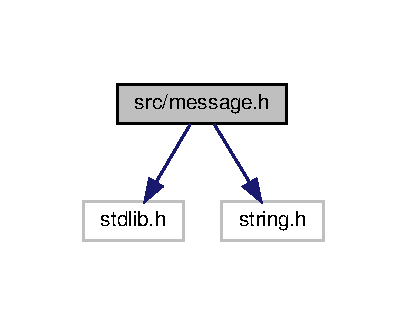
\includegraphics[width=196pt]{message_8h__incl}
\end{center}
\end{figure}
This graph shows which files directly or indirectly include this file\+:\nopagebreak
\begin{figure}[H]
\begin{center}
\leavevmode
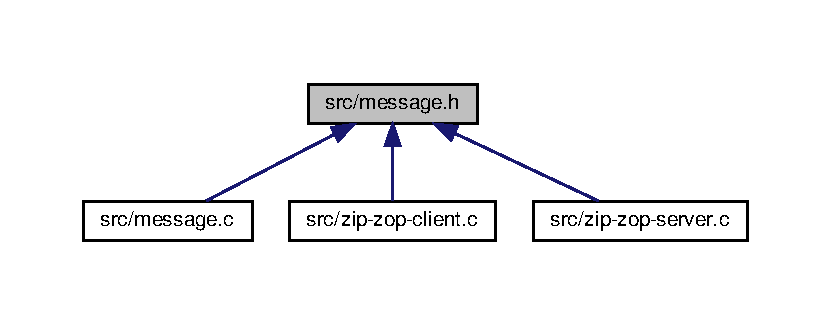
\includegraphics[width=350pt]{message_8h__dep__incl}
\end{center}
\end{figure}
\subsection*{Functions}
\begin{DoxyCompactItemize}
\item 
struct \hyperlink{structmessage}{message} $\ast$ \hyperlink{message_8h_af0270eefb03058e936215fd11fde4b93}{message\+\_\+create} (const char $\ast$content, const char $\ast$sender\+\_\+name)
\begin{DoxyCompactList}\small\item\em Creates a message. \end{DoxyCompactList}\item 
void \hyperlink{message_8h_ad0eaa8623d0f22248ec230fd91bd819b}{message\+\_\+destroy} (struct \hyperlink{structmessage}{message} $\ast$m)
\begin{DoxyCompactList}\small\item\em Destroys a message. \end{DoxyCompactList}\item 
const char $\ast$ \hyperlink{message_8h_a31cd31a7acd86c44c38238f5a5b1da76}{message\+\_\+get\+\_\+content} (struct \hyperlink{structmessage}{message} $\ast$m)
\begin{DoxyCompactList}\small\item\em Get the message content. \end{DoxyCompactList}\item 
const char $\ast$ \hyperlink{message_8h_ac6e3d955212965dc1ab7b5e3f88bc535}{message\+\_\+get\+\_\+sender} (struct \hyperlink{structmessage}{message} $\ast$m)
\begin{DoxyCompactList}\small\item\em Get the message sender. \end{DoxyCompactList}\item 
char $\ast$ \hyperlink{message_8h_a0e07715664284f7a821216ca83317e60}{message\+\_\+pack} (struct \hyperlink{structmessage}{message} $\ast$m, int $\ast$len)
\begin{DoxyCompactList}\small\item\em Serialize a message. \end{DoxyCompactList}\item 
struct \hyperlink{structmessage}{message} $\ast$ \hyperlink{message_8h_a3ba54a38dd0b04dea973f33437bb9125}{message\+\_\+unpack} (char $\ast$pack)
\begin{DoxyCompactList}\small\item\em Deserialize a message. \end{DoxyCompactList}\end{DoxyCompactItemize}


\subsection{Function Documentation}
\mbox{\Hypertarget{message_8h_af0270eefb03058e936215fd11fde4b93}\label{message_8h_af0270eefb03058e936215fd11fde4b93}} 
\index{message.\+h@{message.\+h}!message\+\_\+create@{message\+\_\+create}}
\index{message\+\_\+create@{message\+\_\+create}!message.\+h@{message.\+h}}
\subsubsection{\texorpdfstring{message\+\_\+create()}{message\_create()}}
{\footnotesize\ttfamily struct \hyperlink{structmessage}{message}$\ast$ message\+\_\+create (\begin{DoxyParamCaption}\item[{const char $\ast$}]{content,  }\item[{const char $\ast$}]{sender\+\_\+name }\end{DoxyParamCaption})}



Creates a message. 

Both parameters will be copied into the message, so the user is free to {\ttfamily free()} the parameters passed to this function if necessary.


\begin{DoxyParams}[1]{Parameters}
\mbox{\tt in}  & {\em content} & The content of the message. \\
\hline
\mbox{\tt in}  & {\em sender\+\_\+name} & The username of the sender.\\
\hline
\end{DoxyParams}
\begin{DoxyReturn}{Returns}
A pointer to a struct message in case of success, N\+U\+LL otherwise. The message must be freed, using \hyperlink{message_8c_ad0eaa8623d0f22248ec230fd91bd819b}{message\+\_\+destroy()}, when is not needed anymore. 
\end{DoxyReturn}
\begin{DoxySeeAlso}{See also}
\hyperlink{message_8c_ad0eaa8623d0f22248ec230fd91bd819b}{message\+\_\+destroy} 
\end{DoxySeeAlso}
\mbox{\Hypertarget{message_8h_ad0eaa8623d0f22248ec230fd91bd819b}\label{message_8h_ad0eaa8623d0f22248ec230fd91bd819b}} 
\index{message.\+h@{message.\+h}!message\+\_\+destroy@{message\+\_\+destroy}}
\index{message\+\_\+destroy@{message\+\_\+destroy}!message.\+h@{message.\+h}}
\subsubsection{\texorpdfstring{message\+\_\+destroy()}{message\_destroy()}}
{\footnotesize\ttfamily void message\+\_\+destroy (\begin{DoxyParamCaption}\item[{struct \hyperlink{structmessage}{message} $\ast$}]{m }\end{DoxyParamCaption})}



Destroys a message. 


\begin{DoxyParams}[1]{Parameters}
\mbox{\tt in}  & {\em m} & A pointer to the message.\\
\hline
\end{DoxyParams}
\begin{DoxySeeAlso}{See also}
\hyperlink{message_8c_af0270eefb03058e936215fd11fde4b93}{message\+\_\+create} 
\end{DoxySeeAlso}
\mbox{\Hypertarget{message_8h_a31cd31a7acd86c44c38238f5a5b1da76}\label{message_8h_a31cd31a7acd86c44c38238f5a5b1da76}} 
\index{message.\+h@{message.\+h}!message\+\_\+get\+\_\+content@{message\+\_\+get\+\_\+content}}
\index{message\+\_\+get\+\_\+content@{message\+\_\+get\+\_\+content}!message.\+h@{message.\+h}}
\subsubsection{\texorpdfstring{message\+\_\+get\+\_\+content()}{message\_get\_content()}}
{\footnotesize\ttfamily const char$\ast$ message\+\_\+get\+\_\+content (\begin{DoxyParamCaption}\item[{struct \hyperlink{structmessage}{message} $\ast$}]{m }\end{DoxyParamCaption})}



Get the message content. 


\begin{DoxyParams}[1]{Parameters}
\mbox{\tt in}  & {\em m} & A pointer to the message.\\
\hline
\end{DoxyParams}
\begin{DoxyReturn}{Returns}
A pointer to the message content.
\end{DoxyReturn}
\begin{DoxyWarning}{Warning}
The returned value should not be freed. 
\end{DoxyWarning}
\mbox{\Hypertarget{message_8h_ac6e3d955212965dc1ab7b5e3f88bc535}\label{message_8h_ac6e3d955212965dc1ab7b5e3f88bc535}} 
\index{message.\+h@{message.\+h}!message\+\_\+get\+\_\+sender@{message\+\_\+get\+\_\+sender}}
\index{message\+\_\+get\+\_\+sender@{message\+\_\+get\+\_\+sender}!message.\+h@{message.\+h}}
\subsubsection{\texorpdfstring{message\+\_\+get\+\_\+sender()}{message\_get\_sender()}}
{\footnotesize\ttfamily const char$\ast$ message\+\_\+get\+\_\+sender (\begin{DoxyParamCaption}\item[{struct \hyperlink{structmessage}{message} $\ast$}]{m }\end{DoxyParamCaption})}



Get the message sender. 


\begin{DoxyParams}[1]{Parameters}
\mbox{\tt in}  & {\em m} & A pointer to the message.\\
\hline
\end{DoxyParams}
\begin{DoxyReturn}{Returns}
A pointer to the sender name.
\end{DoxyReturn}
\begin{DoxyWarning}{Warning}
The returned value should not be freed. 
\end{DoxyWarning}
\mbox{\Hypertarget{message_8h_a0e07715664284f7a821216ca83317e60}\label{message_8h_a0e07715664284f7a821216ca83317e60}} 
\index{message.\+h@{message.\+h}!message\+\_\+pack@{message\+\_\+pack}}
\index{message\+\_\+pack@{message\+\_\+pack}!message.\+h@{message.\+h}}
\subsubsection{\texorpdfstring{message\+\_\+pack()}{message\_pack()}}
{\footnotesize\ttfamily char$\ast$ message\+\_\+pack (\begin{DoxyParamCaption}\item[{struct \hyperlink{structmessage}{message} $\ast$}]{m,  }\item[{int $\ast$}]{len }\end{DoxyParamCaption})}



Serialize a message. 

Pack/\+Serialize the struct message in a format that can be sent through the network.


\begin{DoxyParams}[1]{Parameters}
\mbox{\tt in}  & {\em m} & A pointer to the message. \\
\hline
\mbox{\tt out}  & {\em len} & A pointer to a integer where the length of the serialized message will be stored.\\
\hline
\end{DoxyParams}
\begin{DoxyReturn}{Returns}
A pointer to the serialized message. This should be freed when is not necessary anymore.
\end{DoxyReturn}
\begin{DoxySeeAlso}{See also}
\hyperlink{message_8c_a3ba54a38dd0b04dea973f33437bb9125}{message\+\_\+unpack} 
\end{DoxySeeAlso}
\mbox{\Hypertarget{message_8h_a3ba54a38dd0b04dea973f33437bb9125}\label{message_8h_a3ba54a38dd0b04dea973f33437bb9125}} 
\index{message.\+h@{message.\+h}!message\+\_\+unpack@{message\+\_\+unpack}}
\index{message\+\_\+unpack@{message\+\_\+unpack}!message.\+h@{message.\+h}}
\subsubsection{\texorpdfstring{message\+\_\+unpack()}{message\_unpack()}}
{\footnotesize\ttfamily struct \hyperlink{structmessage}{message}$\ast$ message\+\_\+unpack (\begin{DoxyParamCaption}\item[{char $\ast$}]{pack }\end{DoxyParamCaption})}



Deserialize a message. 

Unpack/\+Deserialize a string into a struct message.


\begin{DoxyParams}[1]{Parameters}
\mbox{\tt in}  & {\em pack} & The string that represent the packed message generated by \hyperlink{message_8c_a0e07715664284f7a821216ca83317e60}{message\+\_\+pack()}.\\
\hline
\end{DoxyParams}
\begin{DoxyReturn}{Returns}
A pointer to the deserialized message. This should be freed when is not necessary anymore.
\end{DoxyReturn}
\begin{DoxySeeAlso}{See also}
\hyperlink{message_8c_a0e07715664284f7a821216ca83317e60}{message\+\_\+pack} 
\end{DoxySeeAlso}

\hypertarget{sllist_8c}{}\section{src/sllist.c File Reference}
\label{sllist_8c}\index{src/sllist.\+c@{src/sllist.\+c}}
{\ttfamily \#include \char`\"{}sllist.\+h\char`\"{}}\newline
Include dependency graph for sllist.\+c\+:\nopagebreak
\begin{figure}[H]
\begin{center}
\leavevmode
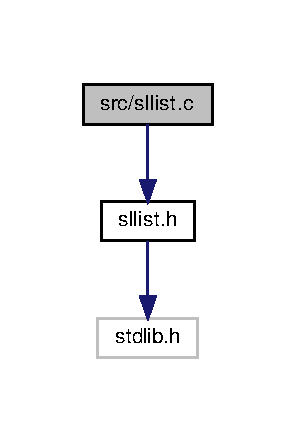
\includegraphics[width=142pt]{sllist_8c__incl}
\end{center}
\end{figure}
\subsection*{Data Structures}
\begin{DoxyCompactItemize}
\item 
struct \hyperlink{structsllist}{sllist}
\begin{DoxyCompactList}\small\item\em A struct representing node in a singly linked list. \end{DoxyCompactList}\end{DoxyCompactItemize}
\subsection*{Functions}
\begin{DoxyCompactItemize}
\item 
struct \hyperlink{structsllist}{sllist} $\ast$ \hyperlink{sllist_8c_ada173d32da00693ac4e803b1343ec4ac}{sll\+\_\+init} (void)
\begin{DoxyCompactList}\small\item\em Initilize a sllist to be a valid empty list. \end{DoxyCompactList}\item 
struct \hyperlink{structsllist}{sllist} $\ast$ \hyperlink{sllist_8c_aa391dba476f2cf8290a77d7445bde246}{sll\+\_\+get\+\_\+next} (struct \hyperlink{structsllist}{sllist} $\ast$$\ast$l)
\begin{DoxyCompactList}\small\item\em Get the next node in the list. \end{DoxyCompactList}\item 
void \hyperlink{sllist_8c_a798d672d70a10222966c9de995496f9f}{sll\+\_\+insert\+\_\+first} (struct \hyperlink{structsllist}{sllist} $\ast$$\ast$l, void $\ast$a)
\begin{DoxyCompactList}\small\item\em Insert an element on the head of the list. \end{DoxyCompactList}\item 
void \hyperlink{sllist_8c_a25e60a1bd89c31e00660743c50aeac87}{sll\+\_\+insert\+\_\+last} (struct \hyperlink{structsllist}{sllist} $\ast$$\ast$l, void $\ast$a)
\begin{DoxyCompactList}\small\item\em Insert an element on the tail of the list. \end{DoxyCompactList}\item 
void $\ast$ \hyperlink{sllist_8c_a3d88e7dea230b8d5854a17f106fb9740}{sll\+\_\+remove\+\_\+first} (struct \hyperlink{structsllist}{sllist} $\ast$$\ast$l)
\begin{DoxyCompactList}\small\item\em Remove the first element of the list. \end{DoxyCompactList}\item 
void $\ast$ \hyperlink{sllist_8c_ab30ebb23c8ba76871885110c64f026f9}{sll\+\_\+remove\+\_\+last} (struct \hyperlink{structsllist}{sllist} $\ast$$\ast$l)
\begin{DoxyCompactList}\small\item\em Remove the last element of the list. \end{DoxyCompactList}\item 
void $\ast$ \hyperlink{sllist_8c_a6a16207cf8ef79ba25ae8e1453ccf0bc}{sll\+\_\+remove\+\_\+elm} (struct \hyperlink{structsllist}{sllist} $\ast$$\ast$l, void $\ast$elm)
\begin{DoxyCompactList}\small\item\em Remove the specified element of the list. \end{DoxyCompactList}\item 
void $\ast$ \hyperlink{sllist_8c_ac2c3278ad40114c39ec8d55e7ffc46b3}{sll\+\_\+get\+\_\+key} (struct \hyperlink{structsllist}{sllist} $\ast$l)
\begin{DoxyCompactList}\small\item\em Get the element stored in the especified list node. \end{DoxyCompactList}\end{DoxyCompactItemize}


\subsection{Function Documentation}
\mbox{\Hypertarget{sllist_8c_ac2c3278ad40114c39ec8d55e7ffc46b3}\label{sllist_8c_ac2c3278ad40114c39ec8d55e7ffc46b3}} 
\index{sllist.\+c@{sllist.\+c}!sll\+\_\+get\+\_\+key@{sll\+\_\+get\+\_\+key}}
\index{sll\+\_\+get\+\_\+key@{sll\+\_\+get\+\_\+key}!sllist.\+c@{sllist.\+c}}
\subsubsection{\texorpdfstring{sll\+\_\+get\+\_\+key()}{sll\_get\_key()}}
{\footnotesize\ttfamily void$\ast$ sll\+\_\+get\+\_\+key (\begin{DoxyParamCaption}\item[{struct \hyperlink{structsllist}{sllist} $\ast$}]{l }\end{DoxyParamCaption})}



Get the element stored in the especified list node. 


\begin{DoxyParams}[1]{Parameters}
\mbox{\tt in}  & {\em l} & A pointer to the list node.\\
\hline
\end{DoxyParams}
\begin{DoxyReturn}{Returns}
The element. 
\end{DoxyReturn}
\mbox{\Hypertarget{sllist_8c_aa391dba476f2cf8290a77d7445bde246}\label{sllist_8c_aa391dba476f2cf8290a77d7445bde246}} 
\index{sllist.\+c@{sllist.\+c}!sll\+\_\+get\+\_\+next@{sll\+\_\+get\+\_\+next}}
\index{sll\+\_\+get\+\_\+next@{sll\+\_\+get\+\_\+next}!sllist.\+c@{sllist.\+c}}
\subsubsection{\texorpdfstring{sll\+\_\+get\+\_\+next()}{sll\_get\_next()}}
{\footnotesize\ttfamily struct \hyperlink{structsllist}{sllist}$\ast$ sll\+\_\+get\+\_\+next (\begin{DoxyParamCaption}\item[{struct \hyperlink{structsllist}{sllist} $\ast$$\ast$}]{l }\end{DoxyParamCaption})}



Get the next node in the list. 


\begin{DoxyParams}[1]{Parameters}
\mbox{\tt in,out}  & {\em l} & An address to a pointer to the list.\\
\hline
\end{DoxyParams}
\begin{DoxyReturn}{Returns}
A pointer to the next node in the list; N\+U\+LL if there is no next element.
\end{DoxyReturn}
Example to interate over a list\+: 
\begin{DoxyCode}
\textcolor{keyword}{struct }\hyperlink{structsllist}{sllist} *l = \hyperlink{sllist_8c_ada173d32da00693ac4e803b1343ec4ac}{sll\_init}();
\textcolor{comment}{// fill the list}
\textcolor{keywordflow}{for} (\textcolor{keyword}{struct} \hyperlink{structsllist}{sllist} *p = l; p; p = \hyperlink{sllist_8c_aa391dba476f2cf8290a77d7445bde246}{sll\_get\_next}(&p)) \{
    \textcolor{keywordtype}{void} *\hyperlink{structsllist_aba6ff88336afdd0d2a8cb0ce396f79b6}{key} = \hyperlink{sllist_8c_ac2c3278ad40114c39ec8d55e7ffc46b3}{sll\_get\_key}(p);
    \textcolor{comment}{// do stuff with p}
\}
\end{DoxyCode}
 \mbox{\Hypertarget{sllist_8c_ada173d32da00693ac4e803b1343ec4ac}\label{sllist_8c_ada173d32da00693ac4e803b1343ec4ac}} 
\index{sllist.\+c@{sllist.\+c}!sll\+\_\+init@{sll\+\_\+init}}
\index{sll\+\_\+init@{sll\+\_\+init}!sllist.\+c@{sllist.\+c}}
\subsubsection{\texorpdfstring{sll\+\_\+init()}{sll\_init()}}
{\footnotesize\ttfamily struct \hyperlink{structsllist}{sllist}$\ast$ sll\+\_\+init (\begin{DoxyParamCaption}\item[{void}]{ }\end{DoxyParamCaption})}



Initilize a sllist to be a valid empty list. 

\begin{DoxyReturn}{Returns}
An empty list.
\end{DoxyReturn}
\begin{DoxyWarning}{Warning}
One should not test the return against N\+U\+LL. N\+U\+LL is the default value. 
\end{DoxyWarning}
\begin{DoxySeeAlso}{See also}
\hyperlink{sllist_8h_a4f1348bb9eb6fe8c2b112e39c1887290}{S\+L\+L\+\_\+\+I\+N\+IT} 
\end{DoxySeeAlso}
\mbox{\Hypertarget{sllist_8c_a798d672d70a10222966c9de995496f9f}\label{sllist_8c_a798d672d70a10222966c9de995496f9f}} 
\index{sllist.\+c@{sllist.\+c}!sll\+\_\+insert\+\_\+first@{sll\+\_\+insert\+\_\+first}}
\index{sll\+\_\+insert\+\_\+first@{sll\+\_\+insert\+\_\+first}!sllist.\+c@{sllist.\+c}}
\subsubsection{\texorpdfstring{sll\+\_\+insert\+\_\+first()}{sll\_insert\_first()}}
{\footnotesize\ttfamily void sll\+\_\+insert\+\_\+first (\begin{DoxyParamCaption}\item[{struct \hyperlink{structsllist}{sllist} $\ast$$\ast$}]{l,  }\item[{void $\ast$}]{a }\end{DoxyParamCaption})}



Insert an element on the head of the list. 


\begin{DoxyParams}[1]{Parameters}
\mbox{\tt in,out}  & {\em l} & An address to a pointer to the list. \\
\hline
\mbox{\tt in}  & {\em a} & The element. \\
\hline
\end{DoxyParams}
\mbox{\Hypertarget{sllist_8c_a25e60a1bd89c31e00660743c50aeac87}\label{sllist_8c_a25e60a1bd89c31e00660743c50aeac87}} 
\index{sllist.\+c@{sllist.\+c}!sll\+\_\+insert\+\_\+last@{sll\+\_\+insert\+\_\+last}}
\index{sll\+\_\+insert\+\_\+last@{sll\+\_\+insert\+\_\+last}!sllist.\+c@{sllist.\+c}}
\subsubsection{\texorpdfstring{sll\+\_\+insert\+\_\+last()}{sll\_insert\_last()}}
{\footnotesize\ttfamily void sll\+\_\+insert\+\_\+last (\begin{DoxyParamCaption}\item[{struct \hyperlink{structsllist}{sllist} $\ast$$\ast$}]{l,  }\item[{void $\ast$}]{a }\end{DoxyParamCaption})}



Insert an element on the tail of the list. 


\begin{DoxyParams}[1]{Parameters}
\mbox{\tt in,out}  & {\em l} & An address to a pointer to the list. \\
\hline
\mbox{\tt in}  & {\em a} & The element. \\
\hline
\end{DoxyParams}
\mbox{\Hypertarget{sllist_8c_a6a16207cf8ef79ba25ae8e1453ccf0bc}\label{sllist_8c_a6a16207cf8ef79ba25ae8e1453ccf0bc}} 
\index{sllist.\+c@{sllist.\+c}!sll\+\_\+remove\+\_\+elm@{sll\+\_\+remove\+\_\+elm}}
\index{sll\+\_\+remove\+\_\+elm@{sll\+\_\+remove\+\_\+elm}!sllist.\+c@{sllist.\+c}}
\subsubsection{\texorpdfstring{sll\+\_\+remove\+\_\+elm()}{sll\_remove\_elm()}}
{\footnotesize\ttfamily void$\ast$ sll\+\_\+remove\+\_\+elm (\begin{DoxyParamCaption}\item[{struct \hyperlink{structsllist}{sllist} $\ast$$\ast$}]{l,  }\item[{void $\ast$}]{elm }\end{DoxyParamCaption})}



Remove the specified element of the list. 


\begin{DoxyParams}[1]{Parameters}
\mbox{\tt in,out}  & {\em l} & An address to a pointer to the list. \\
\hline
\mbox{\tt in}  & {\em elm} & The element.\\
\hline
\end{DoxyParams}
\begin{DoxyReturn}{Returns}
The element in case of success. N\+U\+LL if the list is empty or the element doesn\textquotesingle{}t exit. 
\end{DoxyReturn}
\mbox{\Hypertarget{sllist_8c_a3d88e7dea230b8d5854a17f106fb9740}\label{sllist_8c_a3d88e7dea230b8d5854a17f106fb9740}} 
\index{sllist.\+c@{sllist.\+c}!sll\+\_\+remove\+\_\+first@{sll\+\_\+remove\+\_\+first}}
\index{sll\+\_\+remove\+\_\+first@{sll\+\_\+remove\+\_\+first}!sllist.\+c@{sllist.\+c}}
\subsubsection{\texorpdfstring{sll\+\_\+remove\+\_\+first()}{sll\_remove\_first()}}
{\footnotesize\ttfamily void$\ast$ sll\+\_\+remove\+\_\+first (\begin{DoxyParamCaption}\item[{struct \hyperlink{structsllist}{sllist} $\ast$$\ast$}]{l }\end{DoxyParamCaption})}



Remove the first element of the list. 

The list node will be freed.


\begin{DoxyParams}[1]{Parameters}
\mbox{\tt in,out}  & {\em l} & An address to a pointer to the list.\\
\hline
\end{DoxyParams}
\begin{DoxyReturn}{Returns}
The element in case of success. N\+U\+LL if the list is empty. 
\end{DoxyReturn}
\mbox{\Hypertarget{sllist_8c_ab30ebb23c8ba76871885110c64f026f9}\label{sllist_8c_ab30ebb23c8ba76871885110c64f026f9}} 
\index{sllist.\+c@{sllist.\+c}!sll\+\_\+remove\+\_\+last@{sll\+\_\+remove\+\_\+last}}
\index{sll\+\_\+remove\+\_\+last@{sll\+\_\+remove\+\_\+last}!sllist.\+c@{sllist.\+c}}
\subsubsection{\texorpdfstring{sll\+\_\+remove\+\_\+last()}{sll\_remove\_last()}}
{\footnotesize\ttfamily void$\ast$ sll\+\_\+remove\+\_\+last (\begin{DoxyParamCaption}\item[{struct \hyperlink{structsllist}{sllist} $\ast$$\ast$}]{l }\end{DoxyParamCaption})}



Remove the last element of the list. 

The list node will be freed.


\begin{DoxyParams}[1]{Parameters}
\mbox{\tt in,out}  & {\em l} & An address to a pointer to the list.\\
\hline
\end{DoxyParams}
\begin{DoxyReturn}{Returns}
The element in case of success. N\+U\+LL if the list is empty. 
\end{DoxyReturn}

\hypertarget{sllist_8h}{}\section{src/sllist.h File Reference}
\label{sllist_8h}\index{src/sllist.\+h@{src/sllist.\+h}}
{\ttfamily \#include $<$stdlib.\+h$>$}\newline
Include dependency graph for sllist.\+h\+:\nopagebreak
\begin{figure}[H]
\begin{center}
\leavevmode
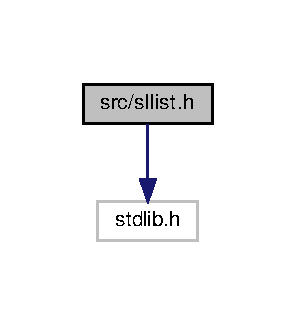
\includegraphics[width=142pt]{sllist_8h__incl}
\end{center}
\end{figure}
This graph shows which files directly or indirectly include this file\+:\nopagebreak
\begin{figure}[H]
\begin{center}
\leavevmode
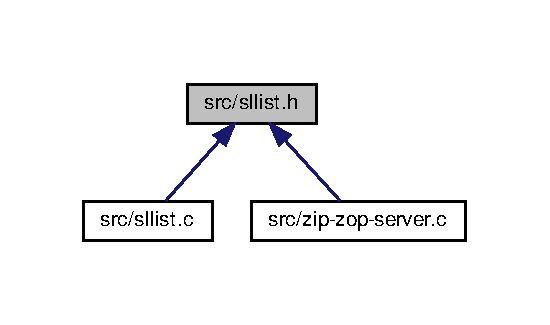
\includegraphics[width=264pt]{sllist_8h__dep__incl}
\end{center}
\end{figure}
\subsection*{Macros}
\begin{DoxyCompactItemize}
\item 
\#define \hyperlink{sllist_8h_a4f1348bb9eb6fe8c2b112e39c1887290}{S\+L\+L\+\_\+\+I\+N\+IT}()~N\+U\+LL;
\begin{DoxyCompactList}\small\item\em Macro that initialize a sllist to be a valid empty list. \end{DoxyCompactList}\end{DoxyCompactItemize}
\subsection*{Functions}
\begin{DoxyCompactItemize}
\item 
struct \hyperlink{structsllist}{sllist} $\ast$ \hyperlink{sllist_8h_ada173d32da00693ac4e803b1343ec4ac}{sll\+\_\+init} (void)
\begin{DoxyCompactList}\small\item\em Initilize a sllist to be a valid empty list. \end{DoxyCompactList}\item 
struct \hyperlink{structsllist}{sllist} $\ast$ \hyperlink{sllist_8h_aa391dba476f2cf8290a77d7445bde246}{sll\+\_\+get\+\_\+next} (struct \hyperlink{structsllist}{sllist} $\ast$$\ast$l)
\begin{DoxyCompactList}\small\item\em Get the next node in the list. \end{DoxyCompactList}\item 
void \hyperlink{sllist_8h_a798d672d70a10222966c9de995496f9f}{sll\+\_\+insert\+\_\+first} (struct \hyperlink{structsllist}{sllist} $\ast$$\ast$l, void $\ast$a)
\begin{DoxyCompactList}\small\item\em Insert an element on the head of the list. \end{DoxyCompactList}\item 
void \hyperlink{sllist_8h_a25e60a1bd89c31e00660743c50aeac87}{sll\+\_\+insert\+\_\+last} (struct \hyperlink{structsllist}{sllist} $\ast$$\ast$l, void $\ast$a)
\begin{DoxyCompactList}\small\item\em Insert an element on the tail of the list. \end{DoxyCompactList}\item 
void $\ast$ \hyperlink{sllist_8h_a3d88e7dea230b8d5854a17f106fb9740}{sll\+\_\+remove\+\_\+first} (struct \hyperlink{structsllist}{sllist} $\ast$$\ast$l)
\begin{DoxyCompactList}\small\item\em Remove the first element of the list. \end{DoxyCompactList}\item 
void $\ast$ \hyperlink{sllist_8h_ab30ebb23c8ba76871885110c64f026f9}{sll\+\_\+remove\+\_\+last} (struct \hyperlink{structsllist}{sllist} $\ast$$\ast$l)
\begin{DoxyCompactList}\small\item\em Remove the last element of the list. \end{DoxyCompactList}\item 
void $\ast$ \hyperlink{sllist_8h_a6a16207cf8ef79ba25ae8e1453ccf0bc}{sll\+\_\+remove\+\_\+elm} (struct \hyperlink{structsllist}{sllist} $\ast$$\ast$l, void $\ast$elm)
\begin{DoxyCompactList}\small\item\em Remove the specified element of the list. \end{DoxyCompactList}\item 
void $\ast$ \hyperlink{sllist_8h_ac2c3278ad40114c39ec8d55e7ffc46b3}{sll\+\_\+get\+\_\+key} (struct \hyperlink{structsllist}{sllist} $\ast$l)
\begin{DoxyCompactList}\small\item\em Get the element stored in the especified list node. \end{DoxyCompactList}\end{DoxyCompactItemize}


\subsection{Macro Definition Documentation}
\mbox{\Hypertarget{sllist_8h_a4f1348bb9eb6fe8c2b112e39c1887290}\label{sllist_8h_a4f1348bb9eb6fe8c2b112e39c1887290}} 
\index{sllist.\+h@{sllist.\+h}!S\+L\+L\+\_\+\+I\+N\+IT@{S\+L\+L\+\_\+\+I\+N\+IT}}
\index{S\+L\+L\+\_\+\+I\+N\+IT@{S\+L\+L\+\_\+\+I\+N\+IT}!sllist.\+h@{sllist.\+h}}
\subsubsection{\texorpdfstring{S\+L\+L\+\_\+\+I\+N\+IT}{SLL\_INIT}}
{\footnotesize\ttfamily \#define S\+L\+L\+\_\+\+I\+N\+IT(\begin{DoxyParamCaption}{ }\end{DoxyParamCaption})~N\+U\+LL;}



Macro that initialize a sllist to be a valid empty list. 

\begin{DoxyReturn}{Returns}
An empty list.
\end{DoxyReturn}
\begin{DoxyWarning}{Warning}
One should not test the return against N\+U\+LL. N\+U\+LL is the default value. 
\end{DoxyWarning}
\begin{DoxySeeAlso}{See also}
\hyperlink{sllist_8h_ada173d32da00693ac4e803b1343ec4ac}{sll\+\_\+init} 
\end{DoxySeeAlso}


\subsection{Function Documentation}
\mbox{\Hypertarget{sllist_8h_ac2c3278ad40114c39ec8d55e7ffc46b3}\label{sllist_8h_ac2c3278ad40114c39ec8d55e7ffc46b3}} 
\index{sllist.\+h@{sllist.\+h}!sll\+\_\+get\+\_\+key@{sll\+\_\+get\+\_\+key}}
\index{sll\+\_\+get\+\_\+key@{sll\+\_\+get\+\_\+key}!sllist.\+h@{sllist.\+h}}
\subsubsection{\texorpdfstring{sll\+\_\+get\+\_\+key()}{sll\_get\_key()}}
{\footnotesize\ttfamily void$\ast$ sll\+\_\+get\+\_\+key (\begin{DoxyParamCaption}\item[{struct \hyperlink{structsllist}{sllist} $\ast$}]{l }\end{DoxyParamCaption})}



Get the element stored in the especified list node. 


\begin{DoxyParams}{Parameters}
{\em l} & A pointer to the list node.\\
\hline
\end{DoxyParams}
\begin{DoxyReturn}{Returns}
The element. 
\end{DoxyReturn}
\mbox{\Hypertarget{sllist_8h_aa391dba476f2cf8290a77d7445bde246}\label{sllist_8h_aa391dba476f2cf8290a77d7445bde246}} 
\index{sllist.\+h@{sllist.\+h}!sll\+\_\+get\+\_\+next@{sll\+\_\+get\+\_\+next}}
\index{sll\+\_\+get\+\_\+next@{sll\+\_\+get\+\_\+next}!sllist.\+h@{sllist.\+h}}
\subsubsection{\texorpdfstring{sll\+\_\+get\+\_\+next()}{sll\_get\_next()}}
{\footnotesize\ttfamily struct \hyperlink{structsllist}{sllist}$\ast$ sll\+\_\+get\+\_\+next (\begin{DoxyParamCaption}\item[{struct \hyperlink{structsllist}{sllist} $\ast$$\ast$}]{l }\end{DoxyParamCaption})}



Get the next node in the list. 


\begin{DoxyParams}{Parameters}
{\em l} & An address to a pointer to the list.\\
\hline
\end{DoxyParams}
\begin{DoxyReturn}{Returns}
A pointer to the next node in the list; N\+U\+LL if there is no next element.
\end{DoxyReturn}
Example to interate over a list\+: 
\begin{DoxyCode}
\textcolor{keyword}{struct }\hyperlink{structsllist}{sllist} **l = \hyperlink{sllist_8c_ada173d32da00693ac4e803b1343ec4ac}{sll\_init}();
\textcolor{comment}{// fill the list}
\textcolor{keywordflow}{for} (\textcolor{keyword}{struct} \hyperlink{structsllist}{sllist} *p = *l; p; p = \hyperlink{sllist_8c_aa391dba476f2cf8290a77d7445bde246}{sll\_get\_next}(&p)) \{
    \textcolor{keywordtype}{void} *\hyperlink{structsllist_aba6ff88336afdd0d2a8cb0ce396f79b6}{key} = \hyperlink{sllist_8c_ac2c3278ad40114c39ec8d55e7ffc46b3}{sll\_get\_key}(p);
    \textcolor{comment}{// do stuff with p}
\}
\end{DoxyCode}
 \mbox{\Hypertarget{sllist_8h_ada173d32da00693ac4e803b1343ec4ac}\label{sllist_8h_ada173d32da00693ac4e803b1343ec4ac}} 
\index{sllist.\+h@{sllist.\+h}!sll\+\_\+init@{sll\+\_\+init}}
\index{sll\+\_\+init@{sll\+\_\+init}!sllist.\+h@{sllist.\+h}}
\subsubsection{\texorpdfstring{sll\+\_\+init()}{sll\_init()}}
{\footnotesize\ttfamily struct \hyperlink{structsllist}{sllist}$\ast$ sll\+\_\+init (\begin{DoxyParamCaption}\item[{void}]{ }\end{DoxyParamCaption})}



Initilize a sllist to be a valid empty list. 

\begin{DoxyReturn}{Returns}
An empty list.
\end{DoxyReturn}
\begin{DoxyWarning}{Warning}
One should not test the return against N\+U\+LL. N\+U\+LL is the default value. 
\end{DoxyWarning}
\begin{DoxySeeAlso}{See also}
\hyperlink{sllist_8h_a4f1348bb9eb6fe8c2b112e39c1887290}{S\+L\+L\+\_\+\+I\+N\+IT} 
\end{DoxySeeAlso}
\mbox{\Hypertarget{sllist_8h_a798d672d70a10222966c9de995496f9f}\label{sllist_8h_a798d672d70a10222966c9de995496f9f}} 
\index{sllist.\+h@{sllist.\+h}!sll\+\_\+insert\+\_\+first@{sll\+\_\+insert\+\_\+first}}
\index{sll\+\_\+insert\+\_\+first@{sll\+\_\+insert\+\_\+first}!sllist.\+h@{sllist.\+h}}
\subsubsection{\texorpdfstring{sll\+\_\+insert\+\_\+first()}{sll\_insert\_first()}}
{\footnotesize\ttfamily void sll\+\_\+insert\+\_\+first (\begin{DoxyParamCaption}\item[{struct \hyperlink{structsllist}{sllist} $\ast$$\ast$}]{l,  }\item[{void $\ast$}]{a }\end{DoxyParamCaption})}



Insert an element on the head of the list. 


\begin{DoxyParams}{Parameters}
{\em l} & An address to a pointer to the list. \\
\hline
{\em a} & The element. \\
\hline
\end{DoxyParams}
\mbox{\Hypertarget{sllist_8h_a25e60a1bd89c31e00660743c50aeac87}\label{sllist_8h_a25e60a1bd89c31e00660743c50aeac87}} 
\index{sllist.\+h@{sllist.\+h}!sll\+\_\+insert\+\_\+last@{sll\+\_\+insert\+\_\+last}}
\index{sll\+\_\+insert\+\_\+last@{sll\+\_\+insert\+\_\+last}!sllist.\+h@{sllist.\+h}}
\subsubsection{\texorpdfstring{sll\+\_\+insert\+\_\+last()}{sll\_insert\_last()}}
{\footnotesize\ttfamily void sll\+\_\+insert\+\_\+last (\begin{DoxyParamCaption}\item[{struct \hyperlink{structsllist}{sllist} $\ast$$\ast$}]{l,  }\item[{void $\ast$}]{a }\end{DoxyParamCaption})}



Insert an element on the tail of the list. 


\begin{DoxyParams}{Parameters}
{\em l} & An address to a pointer to the list. \\
\hline
{\em a} & The element. \\
\hline
\end{DoxyParams}
\mbox{\Hypertarget{sllist_8h_a6a16207cf8ef79ba25ae8e1453ccf0bc}\label{sllist_8h_a6a16207cf8ef79ba25ae8e1453ccf0bc}} 
\index{sllist.\+h@{sllist.\+h}!sll\+\_\+remove\+\_\+elm@{sll\+\_\+remove\+\_\+elm}}
\index{sll\+\_\+remove\+\_\+elm@{sll\+\_\+remove\+\_\+elm}!sllist.\+h@{sllist.\+h}}
\subsubsection{\texorpdfstring{sll\+\_\+remove\+\_\+elm()}{sll\_remove\_elm()}}
{\footnotesize\ttfamily void$\ast$ sll\+\_\+remove\+\_\+elm (\begin{DoxyParamCaption}\item[{struct \hyperlink{structsllist}{sllist} $\ast$$\ast$}]{l,  }\item[{void $\ast$}]{elm }\end{DoxyParamCaption})}



Remove the specified element of the list. 


\begin{DoxyParams}{Parameters}
{\em l} & An address to a pointer to the list. \\
\hline
{\em elm} & The element.\\
\hline
\end{DoxyParams}
\begin{DoxyReturn}{Returns}
The element in case of success. N\+U\+LL if the list is empty or the element doesn\textquotesingle{}t exit. 
\end{DoxyReturn}
\mbox{\Hypertarget{sllist_8h_a3d88e7dea230b8d5854a17f106fb9740}\label{sllist_8h_a3d88e7dea230b8d5854a17f106fb9740}} 
\index{sllist.\+h@{sllist.\+h}!sll\+\_\+remove\+\_\+first@{sll\+\_\+remove\+\_\+first}}
\index{sll\+\_\+remove\+\_\+first@{sll\+\_\+remove\+\_\+first}!sllist.\+h@{sllist.\+h}}
\subsubsection{\texorpdfstring{sll\+\_\+remove\+\_\+first()}{sll\_remove\_first()}}
{\footnotesize\ttfamily void$\ast$ sll\+\_\+remove\+\_\+first (\begin{DoxyParamCaption}\item[{struct \hyperlink{structsllist}{sllist} $\ast$$\ast$}]{l }\end{DoxyParamCaption})}



Remove the first element of the list. 

The list node will be freed.


\begin{DoxyParams}{Parameters}
{\em l} & An address to a pointer to the list.\\
\hline
\end{DoxyParams}
\begin{DoxyReturn}{Returns}
The element in case of success. N\+U\+LL if the list is empty. 
\end{DoxyReturn}
\mbox{\Hypertarget{sllist_8h_ab30ebb23c8ba76871885110c64f026f9}\label{sllist_8h_ab30ebb23c8ba76871885110c64f026f9}} 
\index{sllist.\+h@{sllist.\+h}!sll\+\_\+remove\+\_\+last@{sll\+\_\+remove\+\_\+last}}
\index{sll\+\_\+remove\+\_\+last@{sll\+\_\+remove\+\_\+last}!sllist.\+h@{sllist.\+h}}
\subsubsection{\texorpdfstring{sll\+\_\+remove\+\_\+last()}{sll\_remove\_last()}}
{\footnotesize\ttfamily void$\ast$ sll\+\_\+remove\+\_\+last (\begin{DoxyParamCaption}\item[{struct \hyperlink{structsllist}{sllist} $\ast$$\ast$}]{l }\end{DoxyParamCaption})}



Remove the last element of the list. 

The list node will be freed.


\begin{DoxyParams}{Parameters}
{\em l} & An address to a pointer to the list.\\
\hline
\end{DoxyParams}
\begin{DoxyReturn}{Returns}
The element in case of success. N\+U\+LL if the list is empty. 
\end{DoxyReturn}

\hypertarget{zip-zop-client_8c}{}\section{src/zip-\/zop-\/client.c File Reference}
\label{zip-zop-client_8c}\index{src/zip-\/zop-\/client.\+c@{src/zip-\/zop-\/client.\+c}}
{\ttfamily \#include $<$stdio.\+h$>$}\newline
{\ttfamily \#include $<$stdlib.\+h$>$}\newline
{\ttfamily \#include $<$string.\+h$>$}\newline
{\ttfamily \#include $<$stdbool.\+h$>$}\newline
{\ttfamily \#include $<$sys/types.\+h$>$}\newline
{\ttfamily \#include $<$sys/socket.\+h$>$}\newline
{\ttfamily \#include $<$netdb.\+h$>$}\newline
{\ttfamily \#include $<$unistd.\+h$>$}\newline
{\ttfamily \#include $<$pthread.\+h$>$}\newline
{\ttfamily \#include \char`\"{}errcodes.\+h\char`\"{}}\newline
{\ttfamily \#include \char`\"{}message.\+h\char`\"{}}\newline
{\ttfamily \#include \char`\"{}client.\+h\char`\"{}}\newline
Include dependency graph for zip-\/zop-\/client.c\+:\nopagebreak
\begin{figure}[H]
\begin{center}
\leavevmode
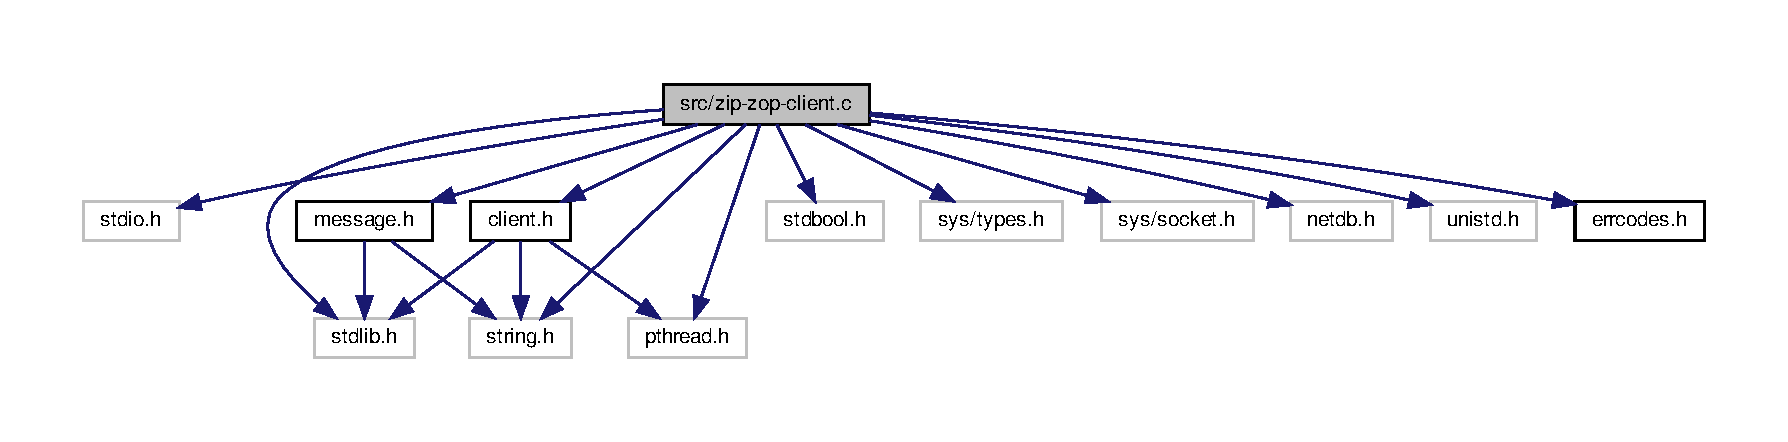
\includegraphics[width=350pt]{zip-zop-client_8c__incl}
\end{center}
\end{figure}
\subsection*{Macros}
\begin{DoxyCompactItemize}
\item 
\#define \hyperlink{zip-zop-client_8c_a614217d263be1fb1a5f76e2ff7be19a2}{P\+O\+RT}~\char`\"{}1234\char`\"{}
\begin{DoxyCompactList}\small\item\em The port where this application will be running. \end{DoxyCompactList}\item 
\#define \hyperlink{zip-zop-client_8c_aa2dfc63100e2bed7efb1b0cd09dea107}{M\+E\+S\+S\+A\+G\+E\+\_\+\+L\+EN}~2000
\begin{DoxyCompactList}\small\item\em Maximum length of a client message. \end{DoxyCompactList}\end{DoxyCompactItemize}
\subsection*{Functions}
\begin{DoxyCompactItemize}
\item 
bool \hyperlink{zip-zop-client_8c_ae42aaff0193542f01451e25d0d0e6725}{check\+\_\+args} (int argc)
\begin{DoxyCompactList}\small\item\em Checks if the user enter the arguments in the correct manner. \end{DoxyCompactList}\item 
void \hyperlink{zip-zop-client_8c_a120fec5c70bad673e9b1c2e91b28fe5f}{print\+\_\+usage} (const char $\ast$name)
\begin{DoxyCompactList}\small\item\em Prints the correct usage of the program. \end{DoxyCompactList}\item 
void \hyperlink{zip-zop-client_8c_aec5550cf115ba01d0da023ba9d1876bb}{show\+\_\+message} (struct \hyperlink{structmessage}{message} $\ast$m)
\begin{DoxyCompactList}\small\item\em Displays a message in the screen. \end{DoxyCompactList}\item 
void $\ast$ \hyperlink{zip-zop-client_8c_aafa1438575f3295609976f35a6518cca}{listen\+\_\+thread} (void $\ast$\hyperlink{structclient}{client})
\begin{DoxyCompactList}\small\item\em Keeps listening to server messages. \end{DoxyCompactList}\item 
void $\ast$ \hyperlink{zip-zop-client_8c_a7ca038c133aa6aca1c539e69d4ee675f}{speak\+\_\+thread} (void $\ast$\hyperlink{structclient}{client})
\begin{DoxyCompactList}\small\item\em Keeps reading messages from {\ttfamily stdin} and send them to server. \end{DoxyCompactList}\item 
struct addrinfo $\ast$ \hyperlink{zip-zop-client_8c_a76840de4643d86b9d0a968ec2d1acae3}{get\+\_\+server\+\_\+addr} (const char $\ast$server\+\_\+name)
\begin{DoxyCompactList}\small\item\em Gets the internet address of the server. \end{DoxyCompactList}\item 
int \hyperlink{zip-zop-client_8c_aff1f8c91603968e32da45fc6ef4bad4d}{create\+\_\+and\+\_\+connect} (struct addrinfo $\ast$addr)
\begin{DoxyCompactList}\small\item\em Attempts to create a socket to an internet address and connect to it in to a port. \end{DoxyCompactList}\item 
void \hyperlink{zip-zop-client_8c_acb0e43d47379736b891394dd383064be}{server\+\_\+introduction} (struct \hyperlink{structclient}{client} $\ast$c)
\begin{DoxyCompactList}\small\item\em Presents the client to the server. \end{DoxyCompactList}\item 
void \hyperlink{zip-zop-client_8c_a1c3a34b362da4351d526c8af94b228c6}{communicate} (const char $\ast$user\+\_\+name, int sockfd)
\begin{DoxyCompactList}\small\item\em Manages the connection with a user and a server. \end{DoxyCompactList}\item 
int \hyperlink{zip-zop-client_8c_a3c04138a5bfe5d72780bb7e82a18e627}{main} (int argc, char $\ast$$\ast$argv)
\begin{DoxyCompactList}\small\item\em The zip-\/zop-\/client. \end{DoxyCompactList}\end{DoxyCompactItemize}


\subsection{Macro Definition Documentation}
\mbox{\Hypertarget{zip-zop-client_8c_aa2dfc63100e2bed7efb1b0cd09dea107}\label{zip-zop-client_8c_aa2dfc63100e2bed7efb1b0cd09dea107}} 
\index{zip-\/zop-\/client.\+c@{zip-\/zop-\/client.\+c}!M\+E\+S\+S\+A\+G\+E\+\_\+\+L\+EN@{M\+E\+S\+S\+A\+G\+E\+\_\+\+L\+EN}}
\index{M\+E\+S\+S\+A\+G\+E\+\_\+\+L\+EN@{M\+E\+S\+S\+A\+G\+E\+\_\+\+L\+EN}!zip-\/zop-\/client.\+c@{zip-\/zop-\/client.\+c}}
\subsubsection{\texorpdfstring{M\+E\+S\+S\+A\+G\+E\+\_\+\+L\+EN}{MESSAGE\_LEN}}
{\footnotesize\ttfamily \#define M\+E\+S\+S\+A\+G\+E\+\_\+\+L\+EN~2000}



Maximum length of a client message. 

\mbox{\Hypertarget{zip-zop-client_8c_a614217d263be1fb1a5f76e2ff7be19a2}\label{zip-zop-client_8c_a614217d263be1fb1a5f76e2ff7be19a2}} 
\index{zip-\/zop-\/client.\+c@{zip-\/zop-\/client.\+c}!P\+O\+RT@{P\+O\+RT}}
\index{P\+O\+RT@{P\+O\+RT}!zip-\/zop-\/client.\+c@{zip-\/zop-\/client.\+c}}
\subsubsection{\texorpdfstring{P\+O\+RT}{PORT}}
{\footnotesize\ttfamily \#define P\+O\+RT~\char`\"{}1234\char`\"{}}



The port where this application will be running. 



\subsection{Function Documentation}
\mbox{\Hypertarget{zip-zop-client_8c_ae42aaff0193542f01451e25d0d0e6725}\label{zip-zop-client_8c_ae42aaff0193542f01451e25d0d0e6725}} 
\index{zip-\/zop-\/client.\+c@{zip-\/zop-\/client.\+c}!check\+\_\+args@{check\+\_\+args}}
\index{check\+\_\+args@{check\+\_\+args}!zip-\/zop-\/client.\+c@{zip-\/zop-\/client.\+c}}
\subsubsection{\texorpdfstring{check\+\_\+args()}{check\_args()}}
{\footnotesize\ttfamily bool check\+\_\+args (\begin{DoxyParamCaption}\item[{int}]{argc }\end{DoxyParamCaption})}



Checks if the user enter the arguments in the correct manner. 


\begin{DoxyParams}[1]{Parameters}
\mbox{\tt in}  & {\em argc} & Number of arguments.\\
\hline
\end{DoxyParams}
\begin{DoxyReturn}{Returns}
{\ttfamily true} if the arguments are correct, {\ttfamily false} otherwise. 
\end{DoxyReturn}
\mbox{\Hypertarget{zip-zop-client_8c_a1c3a34b362da4351d526c8af94b228c6}\label{zip-zop-client_8c_a1c3a34b362da4351d526c8af94b228c6}} 
\index{zip-\/zop-\/client.\+c@{zip-\/zop-\/client.\+c}!communicate@{communicate}}
\index{communicate@{communicate}!zip-\/zop-\/client.\+c@{zip-\/zop-\/client.\+c}}
\subsubsection{\texorpdfstring{communicate()}{communicate()}}
{\footnotesize\ttfamily void communicate (\begin{DoxyParamCaption}\item[{const char $\ast$}]{user\+\_\+name,  }\item[{int}]{sockfd }\end{DoxyParamCaption})}



Manages the connection with a user and a server. 

Given a username and a socket connected with the server, manages the connection, creating a thread to listen to incomming messages from the server, and another to read messages from the user and send them to the server.


\begin{DoxyParams}[1]{Parameters}
\mbox{\tt in}  & {\em user\+\_\+name} & The username. \\
\hline
\mbox{\tt in}  & {\em sockfd} & The socket connected to the server. \\
\hline
\end{DoxyParams}
\mbox{\Hypertarget{zip-zop-client_8c_aff1f8c91603968e32da45fc6ef4bad4d}\label{zip-zop-client_8c_aff1f8c91603968e32da45fc6ef4bad4d}} 
\index{zip-\/zop-\/client.\+c@{zip-\/zop-\/client.\+c}!create\+\_\+and\+\_\+connect@{create\+\_\+and\+\_\+connect}}
\index{create\+\_\+and\+\_\+connect@{create\+\_\+and\+\_\+connect}!zip-\/zop-\/client.\+c@{zip-\/zop-\/client.\+c}}
\subsubsection{\texorpdfstring{create\+\_\+and\+\_\+connect()}{create\_and\_connect()}}
{\footnotesize\ttfamily int create\+\_\+and\+\_\+connect (\begin{DoxyParamCaption}\item[{struct addrinfo $\ast$}]{addr }\end{DoxyParamCaption})}



Attempts to create a socket to an internet address and connect to it in to a port. 


\begin{DoxyParams}[1]{Parameters}
\mbox{\tt in}  & {\em addr} & The internet address.\\
\hline
\end{DoxyParams}
\begin{DoxyReturn}{Returns}
The socket in case os success. {\ttfamily -\/1} otherwise. 
\end{DoxyReturn}
\mbox{\Hypertarget{zip-zop-client_8c_a76840de4643d86b9d0a968ec2d1acae3}\label{zip-zop-client_8c_a76840de4643d86b9d0a968ec2d1acae3}} 
\index{zip-\/zop-\/client.\+c@{zip-\/zop-\/client.\+c}!get\+\_\+server\+\_\+addr@{get\+\_\+server\+\_\+addr}}
\index{get\+\_\+server\+\_\+addr@{get\+\_\+server\+\_\+addr}!zip-\/zop-\/client.\+c@{zip-\/zop-\/client.\+c}}
\subsubsection{\texorpdfstring{get\+\_\+server\+\_\+addr()}{get\_server\_addr()}}
{\footnotesize\ttfamily struct addrinfo$\ast$ get\+\_\+server\+\_\+addr (\begin{DoxyParamCaption}\item[{const char $\ast$}]{server\+\_\+name }\end{DoxyParamCaption})}



Gets the internet address of the server. 

Given the server name, this function will try to find an internet address to this server.


\begin{DoxyParams}[1]{Parameters}
\mbox{\tt in}  & {\em server\+\_\+name} & The server name.\\
\hline
\end{DoxyParams}
\begin{DoxyReturn}{Returns}
A pointer to a list of possibly valid server internet addresses. 
\end{DoxyReturn}
\mbox{\Hypertarget{zip-zop-client_8c_aafa1438575f3295609976f35a6518cca}\label{zip-zop-client_8c_aafa1438575f3295609976f35a6518cca}} 
\index{zip-\/zop-\/client.\+c@{zip-\/zop-\/client.\+c}!listen\+\_\+thread@{listen\+\_\+thread}}
\index{listen\+\_\+thread@{listen\+\_\+thread}!zip-\/zop-\/client.\+c@{zip-\/zop-\/client.\+c}}
\subsubsection{\texorpdfstring{listen\+\_\+thread()}{listen\_thread()}}
{\footnotesize\ttfamily void$\ast$ listen\+\_\+thread (\begin{DoxyParamCaption}\item[{void $\ast$}]{client }\end{DoxyParamCaption})}



Keeps listening to server messages. 

This function will be executed by a thread that is responsable for keep checking if there is a new message from the server.

If there is an new message, the thread will display the message.


\begin{DoxyParams}[1]{Parameters}
\mbox{\tt in}  & {\em client} & A pointer to the client.\\
\hline
\end{DoxyParams}
\begin{DoxySeeAlso}{See also}
\hyperlink{zip-zop-client_8c_aec5550cf115ba01d0da023ba9d1876bb}{show\+\_\+message} 
\end{DoxySeeAlso}
\mbox{\Hypertarget{zip-zop-client_8c_a3c04138a5bfe5d72780bb7e82a18e627}\label{zip-zop-client_8c_a3c04138a5bfe5d72780bb7e82a18e627}} 
\index{zip-\/zop-\/client.\+c@{zip-\/zop-\/client.\+c}!main@{main}}
\index{main@{main}!zip-\/zop-\/client.\+c@{zip-\/zop-\/client.\+c}}
\subsubsection{\texorpdfstring{main()}{main()}}
{\footnotesize\ttfamily int main (\begin{DoxyParamCaption}\item[{int}]{argc,  }\item[{char $\ast$$\ast$}]{argv }\end{DoxyParamCaption})}



The zip-\/zop-\/client. 

A T\+CP client that will connect with an instance of the zip-\/zop-\/server.


\begin{DoxyParams}[1]{Parameters}
\mbox{\tt in}  & {\em argc} & Number of arguments given by the user. \\
\hline
\mbox{\tt in}  & {\em argc} & An array of strings representing the arguments given by the user\\
\hline
\end{DoxyParams}
\begin{DoxyNote}{Note}
Usage\+: ./zip-\/zop-\/client $<$server\+\_\+addr$>$ $<$username$>$ 
\end{DoxyNote}
\mbox{\Hypertarget{zip-zop-client_8c_a120fec5c70bad673e9b1c2e91b28fe5f}\label{zip-zop-client_8c_a120fec5c70bad673e9b1c2e91b28fe5f}} 
\index{zip-\/zop-\/client.\+c@{zip-\/zop-\/client.\+c}!print\+\_\+usage@{print\+\_\+usage}}
\index{print\+\_\+usage@{print\+\_\+usage}!zip-\/zop-\/client.\+c@{zip-\/zop-\/client.\+c}}
\subsubsection{\texorpdfstring{print\+\_\+usage()}{print\_usage()}}
{\footnotesize\ttfamily void print\+\_\+usage (\begin{DoxyParamCaption}\item[{const char $\ast$}]{name }\end{DoxyParamCaption})}



Prints the correct usage of the program. 


\begin{DoxyParams}[1]{Parameters}
\mbox{\tt in}  & {\em name} & The name of this program. \\
\hline
\end{DoxyParams}
\mbox{\Hypertarget{zip-zop-client_8c_acb0e43d47379736b891394dd383064be}\label{zip-zop-client_8c_acb0e43d47379736b891394dd383064be}} 
\index{zip-\/zop-\/client.\+c@{zip-\/zop-\/client.\+c}!server\+\_\+introduction@{server\+\_\+introduction}}
\index{server\+\_\+introduction@{server\+\_\+introduction}!zip-\/zop-\/client.\+c@{zip-\/zop-\/client.\+c}}
\subsubsection{\texorpdfstring{server\+\_\+introduction()}{server\_introduction()}}
{\footnotesize\ttfamily void server\+\_\+introduction (\begin{DoxyParamCaption}\item[{struct \hyperlink{structclient}{client} $\ast$}]{c }\end{DoxyParamCaption})}



Presents the client to the server. 

This function sends everything that is needed to introduce the client to the server.

In this case only the client name is sent to the server.


\begin{DoxyParams}{Parameters}
{\em c} & The client. \\
\hline
\end{DoxyParams}
\mbox{\Hypertarget{zip-zop-client_8c_aec5550cf115ba01d0da023ba9d1876bb}\label{zip-zop-client_8c_aec5550cf115ba01d0da023ba9d1876bb}} 
\index{zip-\/zop-\/client.\+c@{zip-\/zop-\/client.\+c}!show\+\_\+message@{show\+\_\+message}}
\index{show\+\_\+message@{show\+\_\+message}!zip-\/zop-\/client.\+c@{zip-\/zop-\/client.\+c}}
\subsubsection{\texorpdfstring{show\+\_\+message()}{show\_message()}}
{\footnotesize\ttfamily void show\+\_\+message (\begin{DoxyParamCaption}\item[{struct \hyperlink{structmessage}{message} $\ast$}]{m }\end{DoxyParamCaption})}



Displays a message in the screen. 


\begin{DoxyParams}[1]{Parameters}
\mbox{\tt in}  & {\em m} & The message. \\
\hline
\end{DoxyParams}
\mbox{\Hypertarget{zip-zop-client_8c_a7ca038c133aa6aca1c539e69d4ee675f}\label{zip-zop-client_8c_a7ca038c133aa6aca1c539e69d4ee675f}} 
\index{zip-\/zop-\/client.\+c@{zip-\/zop-\/client.\+c}!speak\+\_\+thread@{speak\+\_\+thread}}
\index{speak\+\_\+thread@{speak\+\_\+thread}!zip-\/zop-\/client.\+c@{zip-\/zop-\/client.\+c}}
\subsubsection{\texorpdfstring{speak\+\_\+thread()}{speak\_thread()}}
{\footnotesize\ttfamily void$\ast$ speak\+\_\+thread (\begin{DoxyParamCaption}\item[{void $\ast$}]{client }\end{DoxyParamCaption})}



Keeps reading messages from {\ttfamily stdin} and send them to server. 

The message will be sent as a packet version of a struct message.


\begin{DoxyParams}[1]{Parameters}
\mbox{\tt in}  & {\em c} & The client that sent the message.\\
\hline
\end{DoxyParams}
\begin{DoxySeeAlso}{See also}
\hyperlink{message_8h_a0e07715664284f7a821216ca83317e60}{message\+\_\+pack} 
\end{DoxySeeAlso}

\hypertarget{zip-zop-server_8c}{}\section{src/zip-\/zop-\/server.c File Reference}
\label{zip-zop-server_8c}\index{src/zip-\/zop-\/server.\+c@{src/zip-\/zop-\/server.\+c}}
{\ttfamily \#include $<$stdio.\+h$>$}\newline
{\ttfamily \#include $<$stdlib.\+h$>$}\newline
{\ttfamily \#include $<$string.\+h$>$}\newline
{\ttfamily \#include $<$stdbool.\+h$>$}\newline
{\ttfamily \#include $<$sys/types.\+h$>$}\newline
{\ttfamily \#include $<$sys/socket.\+h$>$}\newline
{\ttfamily \#include $<$netdb.\+h$>$}\newline
{\ttfamily \#include $<$unistd.\+h$>$}\newline
{\ttfamily \#include $<$pthread.\+h$>$}\newline
{\ttfamily \#include \char`\"{}errcodes.\+h\char`\"{}}\newline
{\ttfamily \#include \char`\"{}message.\+h\char`\"{}}\newline
{\ttfamily \#include \char`\"{}client.\+h\char`\"{}}\newline
{\ttfamily \#include \char`\"{}sllist.\+h\char`\"{}}\newline
Include dependency graph for zip-\/zop-\/server.c\+:\nopagebreak
\begin{figure}[H]
\begin{center}
\leavevmode
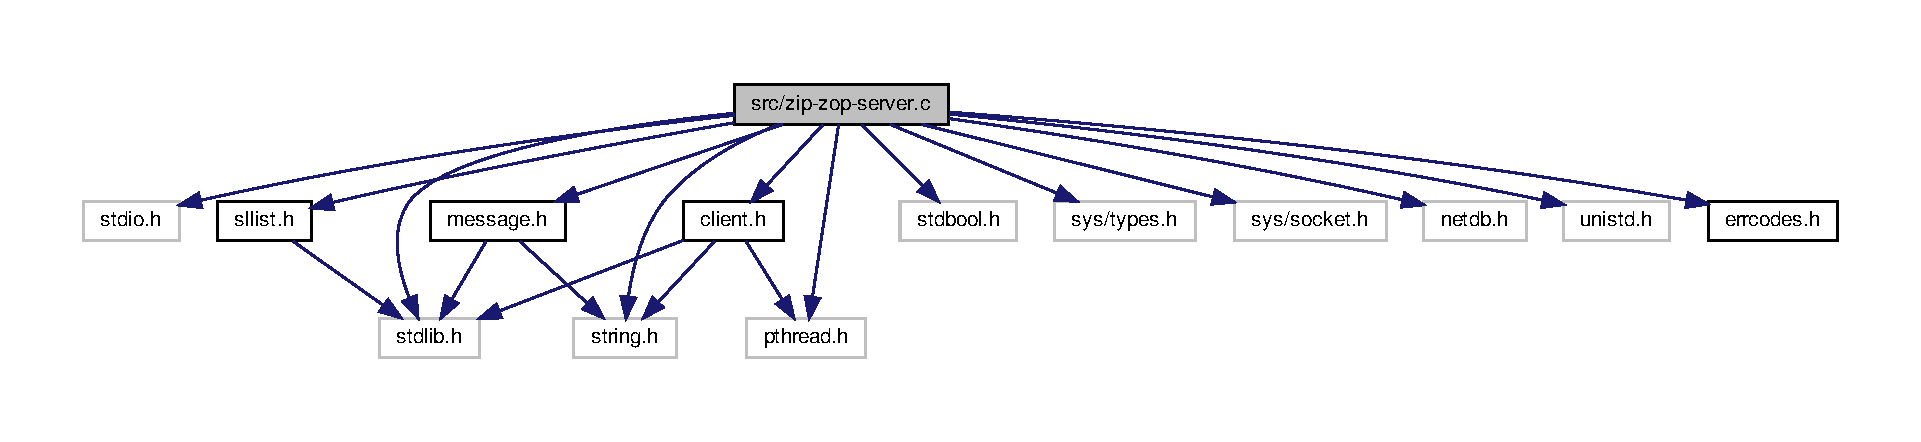
\includegraphics[width=350pt]{zip-zop-server_8c__incl}
\end{center}
\end{figure}
\subsection*{Macros}
\begin{DoxyCompactItemize}
\item 
\#define \hyperlink{zip-zop-server_8c_a614217d263be1fb1a5f76e2ff7be19a2}{P\+O\+RT}~\char`\"{}1234\char`\"{}
\begin{DoxyCompactList}\small\item\em The port where this application will be running. \end{DoxyCompactList}\item 
\#define \hyperlink{zip-zop-server_8c_aeefbbafa97642defe3ee6c3080b7d66f}{B\+A\+C\+K\+L\+OG}~10
\begin{DoxyCompactList}\small\item\em The number of clients that will be kept in the queue if the server is not ready for accepting them. \end{DoxyCompactList}\item 
\#define \hyperlink{zip-zop-server_8c_a2966c973ff2fbc59d762420ad283e82f}{C\+L\+I\+E\+N\+T\+\_\+\+N\+A\+M\+E\+\_\+\+L\+EN}~100
\begin{DoxyCompactList}\small\item\em Maximum length of a client name. \end{DoxyCompactList}\item 
\#define \hyperlink{zip-zop-server_8c_aa2dfc63100e2bed7efb1b0cd09dea107}{M\+E\+S\+S\+A\+G\+E\+\_\+\+L\+EN}~2000
\begin{DoxyCompactList}\small\item\em Maximum length of a client message. \end{DoxyCompactList}\end{DoxyCompactItemize}
\subsection*{Functions}
\begin{DoxyCompactItemize}
\item 
void \hyperlink{zip-zop-server_8c_a84f39912128d6dc7a66bbdd88fad00b5}{insert\+\_\+client\+\_\+concurrent} (struct \hyperlink{structclient}{client} $\ast$c)
\begin{DoxyCompactList}\small\item\em Carry out mutual exclusion and insert the new client on the list. \end{DoxyCompactList}\item 
struct \hyperlink{structclient}{client} $\ast$ \hyperlink{zip-zop-server_8c_a37f14ecc30cc2b45249b544fe70f2b6d}{remove\+\_\+client\+\_\+concurrent} (struct \hyperlink{structclient}{client} $\ast$c)
\begin{DoxyCompactList}\small\item\em Carry out mutual exclusion and remove the new client on the list. \end{DoxyCompactList}\item 
void \hyperlink{zip-zop-server_8c_a36e911ded647a0697ca152cae890bcf5}{broadcast\+\_\+client\+\_\+message} (struct \hyperlink{structclient}{client} $\ast$c, const char $\ast$msg)
\begin{DoxyCompactList}\small\item\em Sends a message to all clients. \end{DoxyCompactList}\item 
void \hyperlink{zip-zop-server_8c_ae5845d7e65c1c7407d1df63105450b5e}{kill\+\_\+client} (struct \hyperlink{structclient}{client} $\ast$c)
\begin{DoxyCompactList}\small\item\em Kill a client. \end{DoxyCompactList}\item 
void $\ast$ \hyperlink{zip-zop-server_8c_abb42bd69f5e5088fef8519780a977f98}{listen\+\_\+to\+\_\+client\+\_\+thread} (void $\ast$\hyperlink{structclient}{client})
\begin{DoxyCompactList}\small\item\em Keeps listening to client messages. \end{DoxyCompactList}\item 
void \hyperlink{zip-zop-server_8c_ab9a14cd690eac9781dd224e034fbd01d}{create\+\_\+new\+\_\+client} (int sockfd)
\begin{DoxyCompactList}\small\item\em Create a new client and add it in the {\ttfamily C\+L\+I\+E\+N\+T\+\_\+\+L\+I\+ST}. \end{DoxyCompactList}\item 
int \hyperlink{zip-zop-server_8c_a8c505192e7c73e767d53f7d282cfb646}{accept\+\_\+clients\+\_\+thread} (void $\ast$sock)
\begin{DoxyCompactList}\small\item\em Keeps on accepting new clients connections. \end{DoxyCompactList}\item 
struct addrinfo $\ast$ \hyperlink{zip-zop-server_8c_a2d9748875d07382b9dbecb97c6cd9b62}{get\+\_\+internet\+\_\+addr} (void)
\begin{DoxyCompactList}\small\item\em Find a set of possible internet addresses of localhost. \end{DoxyCompactList}\item 
int \hyperlink{zip-zop-server_8c_a0ecdeaf556729d827a07915b7a89866c}{create\+\_\+and\+\_\+bind} (struct addrinfo $\ast$addr)
\begin{DoxyCompactList}\small\item\em Attempts to create a socket and bind to a port with the given internet address. \end{DoxyCompactList}\item 
int \hyperlink{zip-zop-server_8c_a59ee6eb284b065353164c1aa7d487ce2}{configure\+\_\+as\+\_\+server} (void)
\begin{DoxyCompactList}\small\item\em This function is responsible to make the initial configuration, so that this program can run as a server. \end{DoxyCompactList}\item 
int \hyperlink{zip-zop-server_8c_a840291bc02cba5474a4cb46a9b9566fe}{main} (void)
\begin{DoxyCompactList}\small\item\em The zip-\/zop-\/server. \end{DoxyCompactList}\end{DoxyCompactItemize}
\subsection*{Variables}
\begin{DoxyCompactItemize}
\item 
struct \hyperlink{structsllist}{sllist} $\ast$ \hyperlink{zip-zop-server_8c_a32076dcdfaf1057a014d74d01cc7e08e}{C\+L\+I\+E\+N\+T\+\_\+\+L\+I\+ST} = \hyperlink{sllist_8h_a4f1348bb9eb6fe8c2b112e39c1887290}{S\+L\+L\+\_\+\+I\+N\+IT}()
\begin{DoxyCompactList}\small\item\em A singly linked list that will keep all the connected clients. \end{DoxyCompactList}\item 
pthread\+\_\+mutex\+\_\+t \hyperlink{zip-zop-server_8c_ac58873310e66c9bfafdbc798a8a7c7e2}{C\+L\+I\+E\+N\+T\+\_\+\+L\+I\+S\+T\+\_\+\+M\+U\+T\+EX}
\begin{DoxyCompactList}\small\item\em The {\ttfamily C\+L\+I\+E\+N\+T\+\_\+\+L\+I\+ST} mutex. \end{DoxyCompactList}\end{DoxyCompactItemize}


\subsection{Macro Definition Documentation}
\mbox{\Hypertarget{zip-zop-server_8c_aeefbbafa97642defe3ee6c3080b7d66f}\label{zip-zop-server_8c_aeefbbafa97642defe3ee6c3080b7d66f}} 
\index{zip-\/zop-\/server.\+c@{zip-\/zop-\/server.\+c}!B\+A\+C\+K\+L\+OG@{B\+A\+C\+K\+L\+OG}}
\index{B\+A\+C\+K\+L\+OG@{B\+A\+C\+K\+L\+OG}!zip-\/zop-\/server.\+c@{zip-\/zop-\/server.\+c}}
\subsubsection{\texorpdfstring{B\+A\+C\+K\+L\+OG}{BACKLOG}}
{\footnotesize\ttfamily \#define B\+A\+C\+K\+L\+OG~10}



The number of clients that will be kept in the queue if the server is not ready for accepting them. 

\mbox{\Hypertarget{zip-zop-server_8c_a2966c973ff2fbc59d762420ad283e82f}\label{zip-zop-server_8c_a2966c973ff2fbc59d762420ad283e82f}} 
\index{zip-\/zop-\/server.\+c@{zip-\/zop-\/server.\+c}!C\+L\+I\+E\+N\+T\+\_\+\+N\+A\+M\+E\+\_\+\+L\+EN@{C\+L\+I\+E\+N\+T\+\_\+\+N\+A\+M\+E\+\_\+\+L\+EN}}
\index{C\+L\+I\+E\+N\+T\+\_\+\+N\+A\+M\+E\+\_\+\+L\+EN@{C\+L\+I\+E\+N\+T\+\_\+\+N\+A\+M\+E\+\_\+\+L\+EN}!zip-\/zop-\/server.\+c@{zip-\/zop-\/server.\+c}}
\subsubsection{\texorpdfstring{C\+L\+I\+E\+N\+T\+\_\+\+N\+A\+M\+E\+\_\+\+L\+EN}{CLIENT\_NAME\_LEN}}
{\footnotesize\ttfamily \#define C\+L\+I\+E\+N\+T\+\_\+\+N\+A\+M\+E\+\_\+\+L\+EN~100}



Maximum length of a client name. 

\mbox{\Hypertarget{zip-zop-server_8c_aa2dfc63100e2bed7efb1b0cd09dea107}\label{zip-zop-server_8c_aa2dfc63100e2bed7efb1b0cd09dea107}} 
\index{zip-\/zop-\/server.\+c@{zip-\/zop-\/server.\+c}!M\+E\+S\+S\+A\+G\+E\+\_\+\+L\+EN@{M\+E\+S\+S\+A\+G\+E\+\_\+\+L\+EN}}
\index{M\+E\+S\+S\+A\+G\+E\+\_\+\+L\+EN@{M\+E\+S\+S\+A\+G\+E\+\_\+\+L\+EN}!zip-\/zop-\/server.\+c@{zip-\/zop-\/server.\+c}}
\subsubsection{\texorpdfstring{M\+E\+S\+S\+A\+G\+E\+\_\+\+L\+EN}{MESSAGE\_LEN}}
{\footnotesize\ttfamily \#define M\+E\+S\+S\+A\+G\+E\+\_\+\+L\+EN~2000}



Maximum length of a client message. 

\mbox{\Hypertarget{zip-zop-server_8c_a614217d263be1fb1a5f76e2ff7be19a2}\label{zip-zop-server_8c_a614217d263be1fb1a5f76e2ff7be19a2}} 
\index{zip-\/zop-\/server.\+c@{zip-\/zop-\/server.\+c}!P\+O\+RT@{P\+O\+RT}}
\index{P\+O\+RT@{P\+O\+RT}!zip-\/zop-\/server.\+c@{zip-\/zop-\/server.\+c}}
\subsubsection{\texorpdfstring{P\+O\+RT}{PORT}}
{\footnotesize\ttfamily \#define P\+O\+RT~\char`\"{}1234\char`\"{}}



The port where this application will be running. 



\subsection{Function Documentation}
\mbox{\Hypertarget{zip-zop-server_8c_a8c505192e7c73e767d53f7d282cfb646}\label{zip-zop-server_8c_a8c505192e7c73e767d53f7d282cfb646}} 
\index{zip-\/zop-\/server.\+c@{zip-\/zop-\/server.\+c}!accept\+\_\+clients\+\_\+thread@{accept\+\_\+clients\+\_\+thread}}
\index{accept\+\_\+clients\+\_\+thread@{accept\+\_\+clients\+\_\+thread}!zip-\/zop-\/server.\+c@{zip-\/zop-\/server.\+c}}
\subsubsection{\texorpdfstring{accept\+\_\+clients\+\_\+thread()}{accept\_clients\_thread()}}
{\footnotesize\ttfamily int accept\+\_\+clients\+\_\+thread (\begin{DoxyParamCaption}\item[{void $\ast$}]{sock }\end{DoxyParamCaption})}



Keeps on accepting new clients connections. 

Keeps listening for incoming connections, wen a new one arrives accepts it and instantiates a new client.


\begin{DoxyParams}[1]{Parameters}
\mbox{\tt in}  & {\em sock} & Adress to the socket used to listen to new connections. \\
\hline
\end{DoxyParams}
\mbox{\Hypertarget{zip-zop-server_8c_a36e911ded647a0697ca152cae890bcf5}\label{zip-zop-server_8c_a36e911ded647a0697ca152cae890bcf5}} 
\index{zip-\/zop-\/server.\+c@{zip-\/zop-\/server.\+c}!broadcast\+\_\+client\+\_\+message@{broadcast\+\_\+client\+\_\+message}}
\index{broadcast\+\_\+client\+\_\+message@{broadcast\+\_\+client\+\_\+message}!zip-\/zop-\/server.\+c@{zip-\/zop-\/server.\+c}}
\subsubsection{\texorpdfstring{broadcast\+\_\+client\+\_\+message()}{broadcast\_client\_message()}}
{\footnotesize\ttfamily void broadcast\+\_\+client\+\_\+message (\begin{DoxyParamCaption}\item[{struct \hyperlink{structclient}{client} $\ast$}]{c,  }\item[{const char $\ast$}]{msg }\end{DoxyParamCaption})}



Sends a message to all clients. 

The message will be sent as a packet version of a struct message.


\begin{DoxyParams}[1]{Parameters}
\mbox{\tt in}  & {\em c} & The client that sent the message. \\
\hline
\mbox{\tt in}  & {\em msg} & The message content.\\
\hline
\end{DoxyParams}
\begin{DoxySeeAlso}{See also}
\hyperlink{message_8h_a0e07715664284f7a821216ca83317e60}{message\+\_\+pack} 
\end{DoxySeeAlso}
\mbox{\Hypertarget{zip-zop-server_8c_a59ee6eb284b065353164c1aa7d487ce2}\label{zip-zop-server_8c_a59ee6eb284b065353164c1aa7d487ce2}} 
\index{zip-\/zop-\/server.\+c@{zip-\/zop-\/server.\+c}!configure\+\_\+as\+\_\+server@{configure\+\_\+as\+\_\+server}}
\index{configure\+\_\+as\+\_\+server@{configure\+\_\+as\+\_\+server}!zip-\/zop-\/server.\+c@{zip-\/zop-\/server.\+c}}
\subsubsection{\texorpdfstring{configure\+\_\+as\+\_\+server()}{configure\_as\_server()}}
{\footnotesize\ttfamily int configure\+\_\+as\+\_\+server (\begin{DoxyParamCaption}\item[{void}]{ }\end{DoxyParamCaption})}



This function is responsible to make the initial configuration, so that this program can run as a server. 

\begin{DoxyReturn}{Returns}
A socket in passive mode, that has the localhost address asigned to it. The user should be able to call accept() in this socket. 
\end{DoxyReturn}
\mbox{\Hypertarget{zip-zop-server_8c_a0ecdeaf556729d827a07915b7a89866c}\label{zip-zop-server_8c_a0ecdeaf556729d827a07915b7a89866c}} 
\index{zip-\/zop-\/server.\+c@{zip-\/zop-\/server.\+c}!create\+\_\+and\+\_\+bind@{create\+\_\+and\+\_\+bind}}
\index{create\+\_\+and\+\_\+bind@{create\+\_\+and\+\_\+bind}!zip-\/zop-\/server.\+c@{zip-\/zop-\/server.\+c}}
\subsubsection{\texorpdfstring{create\+\_\+and\+\_\+bind()}{create\_and\_bind()}}
{\footnotesize\ttfamily int create\+\_\+and\+\_\+bind (\begin{DoxyParamCaption}\item[{struct addrinfo $\ast$}]{addr }\end{DoxyParamCaption})}



Attempts to create a socket and bind to a port with the given internet address. 


\begin{DoxyParams}[1]{Parameters}
\mbox{\tt in}  & {\em addr} & The internet address.\\
\hline
\end{DoxyParams}
\begin{DoxyReturn}{Returns}
The socket in case os success. {\ttfamily -\/1} otherwise. 
\end{DoxyReturn}
\mbox{\Hypertarget{zip-zop-server_8c_ab9a14cd690eac9781dd224e034fbd01d}\label{zip-zop-server_8c_ab9a14cd690eac9781dd224e034fbd01d}} 
\index{zip-\/zop-\/server.\+c@{zip-\/zop-\/server.\+c}!create\+\_\+new\+\_\+client@{create\+\_\+new\+\_\+client}}
\index{create\+\_\+new\+\_\+client@{create\+\_\+new\+\_\+client}!zip-\/zop-\/server.\+c@{zip-\/zop-\/server.\+c}}
\subsubsection{\texorpdfstring{create\+\_\+new\+\_\+client()}{create\_new\_client()}}
{\footnotesize\ttfamily void create\+\_\+new\+\_\+client (\begin{DoxyParamCaption}\item[{int}]{sockfd }\end{DoxyParamCaption})}



Create a new client and add it in the {\ttfamily C\+L\+I\+E\+N\+T\+\_\+\+L\+I\+ST}. 

Also broadcast everyone that the new client has entered the room.


\begin{DoxyParams}[1]{Parameters}
\mbox{\tt in}  & {\em sockfd} & The socket created in \hyperlink{zip-zop-server_8c_a8c505192e7c73e767d53f7d282cfb646}{accept\+\_\+clients\+\_\+thread()}, and that is used to communicate with the client that will be created.\\
\hline
\end{DoxyParams}
\begin{DoxySeeAlso}{See also}
\hyperlink{zip-zop-server_8c_a8c505192e7c73e767d53f7d282cfb646}{accept\+\_\+clients\+\_\+thread} 

\hyperlink{zip-zop-server_8c_a32076dcdfaf1057a014d74d01cc7e08e}{C\+L\+I\+E\+N\+T\+\_\+\+L\+I\+ST} 
\end{DoxySeeAlso}
\mbox{\Hypertarget{zip-zop-server_8c_a2d9748875d07382b9dbecb97c6cd9b62}\label{zip-zop-server_8c_a2d9748875d07382b9dbecb97c6cd9b62}} 
\index{zip-\/zop-\/server.\+c@{zip-\/zop-\/server.\+c}!get\+\_\+internet\+\_\+addr@{get\+\_\+internet\+\_\+addr}}
\index{get\+\_\+internet\+\_\+addr@{get\+\_\+internet\+\_\+addr}!zip-\/zop-\/server.\+c@{zip-\/zop-\/server.\+c}}
\subsubsection{\texorpdfstring{get\+\_\+internet\+\_\+addr()}{get\_internet\_addr()}}
{\footnotesize\ttfamily struct addrinfo$\ast$ get\+\_\+internet\+\_\+addr (\begin{DoxyParamCaption}\item[{void}]{ }\end{DoxyParamCaption})}



Find a set of possible internet addresses of localhost. 

\begin{DoxyReturn}{Returns}
A list of addrinfo, wich contain the adresses. 
\end{DoxyReturn}
\mbox{\Hypertarget{zip-zop-server_8c_a84f39912128d6dc7a66bbdd88fad00b5}\label{zip-zop-server_8c_a84f39912128d6dc7a66bbdd88fad00b5}} 
\index{zip-\/zop-\/server.\+c@{zip-\/zop-\/server.\+c}!insert\+\_\+client\+\_\+concurrent@{insert\+\_\+client\+\_\+concurrent}}
\index{insert\+\_\+client\+\_\+concurrent@{insert\+\_\+client\+\_\+concurrent}!zip-\/zop-\/server.\+c@{zip-\/zop-\/server.\+c}}
\subsubsection{\texorpdfstring{insert\+\_\+client\+\_\+concurrent()}{insert\_client\_concurrent()}}
{\footnotesize\ttfamily void insert\+\_\+client\+\_\+concurrent (\begin{DoxyParamCaption}\item[{struct \hyperlink{structclient}{client} $\ast$}]{c }\end{DoxyParamCaption})}



Carry out mutual exclusion and insert the new client on the list. 

This function locks the {\ttfamily C\+L\+I\+E\+N\+T\+\_\+\+L\+I\+S\+T\+\_\+\+M\+U\+T\+EX} and inserts the client on the list, then unlocks the mutex.


\begin{DoxyParams}[1]{Parameters}
\mbox{\tt in}  & {\em c} & The client.\\
\hline
\end{DoxyParams}
\begin{DoxySeeAlso}{See also}
\hyperlink{zip-zop-server_8c_a32076dcdfaf1057a014d74d01cc7e08e}{C\+L\+I\+E\+N\+T\+\_\+\+L\+I\+ST} 

\hyperlink{zip-zop-server_8c_ac58873310e66c9bfafdbc798a8a7c7e2}{C\+L\+I\+E\+N\+T\+\_\+\+L\+I\+S\+T\+\_\+\+M\+U\+T\+EX} 
\end{DoxySeeAlso}
\mbox{\Hypertarget{zip-zop-server_8c_ae5845d7e65c1c7407d1df63105450b5e}\label{zip-zop-server_8c_ae5845d7e65c1c7407d1df63105450b5e}} 
\index{zip-\/zop-\/server.\+c@{zip-\/zop-\/server.\+c}!kill\+\_\+client@{kill\+\_\+client}}
\index{kill\+\_\+client@{kill\+\_\+client}!zip-\/zop-\/server.\+c@{zip-\/zop-\/server.\+c}}
\subsubsection{\texorpdfstring{kill\+\_\+client()}{kill\_client()}}
{\footnotesize\ttfamily void kill\+\_\+client (\begin{DoxyParamCaption}\item[{struct \hyperlink{structclient}{client} $\ast$}]{c }\end{DoxyParamCaption})}



Kill a client. 

Removes a client from the {\ttfamily C\+L\+I\+E\+N\+T\+\_\+\+L\+I\+ST}, destroys it and closes the connection.


\begin{DoxyParams}[1]{Parameters}
\mbox{\tt in}  & {\em c} & The client.\\
\hline
\end{DoxyParams}
\begin{DoxySeeAlso}{See also}
\hyperlink{zip-zop-server_8c_a32076dcdfaf1057a014d74d01cc7e08e}{C\+L\+I\+E\+N\+T\+\_\+\+L\+I\+ST} 
\end{DoxySeeAlso}
\mbox{\Hypertarget{zip-zop-server_8c_abb42bd69f5e5088fef8519780a977f98}\label{zip-zop-server_8c_abb42bd69f5e5088fef8519780a977f98}} 
\index{zip-\/zop-\/server.\+c@{zip-\/zop-\/server.\+c}!listen\+\_\+to\+\_\+client\+\_\+thread@{listen\+\_\+to\+\_\+client\+\_\+thread}}
\index{listen\+\_\+to\+\_\+client\+\_\+thread@{listen\+\_\+to\+\_\+client\+\_\+thread}!zip-\/zop-\/server.\+c@{zip-\/zop-\/server.\+c}}
\subsubsection{\texorpdfstring{listen\+\_\+to\+\_\+client\+\_\+thread()}{listen\_to\_client\_thread()}}
{\footnotesize\ttfamily void$\ast$ listen\+\_\+to\+\_\+client\+\_\+thread (\begin{DoxyParamCaption}\item[{void $\ast$}]{client }\end{DoxyParamCaption})}



Keeps listening to client messages. 

This function will be executed by a thread that is responsable for keep checking if there is a new message from the client.

If there is an new message, the thread will execute the \hyperlink{zip-zop-server_8c_a36e911ded647a0697ca152cae890bcf5}{broadcast\+\_\+client\+\_\+message()}.


\begin{DoxyParams}[1]{Parameters}
\mbox{\tt in}  & {\em client} & A pointer to the client.\\
\hline
\end{DoxyParams}
\begin{DoxySeeAlso}{See also}
\hyperlink{zip-zop-server_8c_a36e911ded647a0697ca152cae890bcf5}{broadcast\+\_\+client\+\_\+message} 
\end{DoxySeeAlso}
\mbox{\Hypertarget{zip-zop-server_8c_a840291bc02cba5474a4cb46a9b9566fe}\label{zip-zop-server_8c_a840291bc02cba5474a4cb46a9b9566fe}} 
\index{zip-\/zop-\/server.\+c@{zip-\/zop-\/server.\+c}!main@{main}}
\index{main@{main}!zip-\/zop-\/server.\+c@{zip-\/zop-\/server.\+c}}
\subsubsection{\texorpdfstring{main()}{main()}}
{\footnotesize\ttfamily int main (\begin{DoxyParamCaption}\item[{void}]{ }\end{DoxyParamCaption})}



The zip-\/zop-\/server. 

A T\+CP server that will accept connections from zip-\/zop-\/clients, hear its messages and broadcast them to all connected clients. Working as a chatroom. \mbox{\Hypertarget{zip-zop-server_8c_a37f14ecc30cc2b45249b544fe70f2b6d}\label{zip-zop-server_8c_a37f14ecc30cc2b45249b544fe70f2b6d}} 
\index{zip-\/zop-\/server.\+c@{zip-\/zop-\/server.\+c}!remove\+\_\+client\+\_\+concurrent@{remove\+\_\+client\+\_\+concurrent}}
\index{remove\+\_\+client\+\_\+concurrent@{remove\+\_\+client\+\_\+concurrent}!zip-\/zop-\/server.\+c@{zip-\/zop-\/server.\+c}}
\subsubsection{\texorpdfstring{remove\+\_\+client\+\_\+concurrent()}{remove\_client\_concurrent()}}
{\footnotesize\ttfamily struct \hyperlink{structclient}{client}$\ast$ remove\+\_\+client\+\_\+concurrent (\begin{DoxyParamCaption}\item[{struct \hyperlink{structclient}{client} $\ast$}]{c }\end{DoxyParamCaption})}



Carry out mutual exclusion and remove the new client on the list. 

This function locks the {\ttfamily C\+L\+I\+E\+N\+T\+\_\+\+L\+I\+S\+T\+\_\+\+M\+U\+T\+EX} and inserts the client on the list, then unlocks the mutex.


\begin{DoxyParams}[1]{Parameters}
\mbox{\tt in}  & {\em c} & The client.\\
\hline
\end{DoxyParams}
\begin{DoxyReturn}{Returns}
The client just removed. N\+U\+LL otherwise.
\end{DoxyReturn}
\begin{DoxySeeAlso}{See also}
\hyperlink{zip-zop-server_8c_a32076dcdfaf1057a014d74d01cc7e08e}{C\+L\+I\+E\+N\+T\+\_\+\+L\+I\+ST} 

\hyperlink{zip-zop-server_8c_ac58873310e66c9bfafdbc798a8a7c7e2}{C\+L\+I\+E\+N\+T\+\_\+\+L\+I\+S\+T\+\_\+\+M\+U\+T\+EX} 
\end{DoxySeeAlso}


\subsection{Variable Documentation}
\mbox{\Hypertarget{zip-zop-server_8c_a32076dcdfaf1057a014d74d01cc7e08e}\label{zip-zop-server_8c_a32076dcdfaf1057a014d74d01cc7e08e}} 
\index{zip-\/zop-\/server.\+c@{zip-\/zop-\/server.\+c}!C\+L\+I\+E\+N\+T\+\_\+\+L\+I\+ST@{C\+L\+I\+E\+N\+T\+\_\+\+L\+I\+ST}}
\index{C\+L\+I\+E\+N\+T\+\_\+\+L\+I\+ST@{C\+L\+I\+E\+N\+T\+\_\+\+L\+I\+ST}!zip-\/zop-\/server.\+c@{zip-\/zop-\/server.\+c}}
\subsubsection{\texorpdfstring{C\+L\+I\+E\+N\+T\+\_\+\+L\+I\+ST}{CLIENT\_LIST}}
{\footnotesize\ttfamily struct \hyperlink{structsllist}{sllist}$\ast$ C\+L\+I\+E\+N\+T\+\_\+\+L\+I\+ST = \hyperlink{sllist_8h_a4f1348bb9eb6fe8c2b112e39c1887290}{S\+L\+L\+\_\+\+I\+N\+IT}()}



A singly linked list that will keep all the connected clients. 

\begin{DoxyWarning}{Warning}
Mutual exclusion must be ensured before accessing this list.
\end{DoxyWarning}
\begin{DoxySeeAlso}{See also}
\hyperlink{zip-zop-server_8c_ac58873310e66c9bfafdbc798a8a7c7e2}{C\+L\+I\+E\+N\+T\+\_\+\+L\+I\+S\+T\+\_\+\+M\+U\+T\+EX} 
\end{DoxySeeAlso}
\mbox{\Hypertarget{zip-zop-server_8c_ac58873310e66c9bfafdbc798a8a7c7e2}\label{zip-zop-server_8c_ac58873310e66c9bfafdbc798a8a7c7e2}} 
\index{zip-\/zop-\/server.\+c@{zip-\/zop-\/server.\+c}!C\+L\+I\+E\+N\+T\+\_\+\+L\+I\+S\+T\+\_\+\+M\+U\+T\+EX@{C\+L\+I\+E\+N\+T\+\_\+\+L\+I\+S\+T\+\_\+\+M\+U\+T\+EX}}
\index{C\+L\+I\+E\+N\+T\+\_\+\+L\+I\+S\+T\+\_\+\+M\+U\+T\+EX@{C\+L\+I\+E\+N\+T\+\_\+\+L\+I\+S\+T\+\_\+\+M\+U\+T\+EX}!zip-\/zop-\/server.\+c@{zip-\/zop-\/server.\+c}}
\subsubsection{\texorpdfstring{C\+L\+I\+E\+N\+T\+\_\+\+L\+I\+S\+T\+\_\+\+M\+U\+T\+EX}{CLIENT\_LIST\_MUTEX}}
{\footnotesize\ttfamily pthread\+\_\+mutex\+\_\+t C\+L\+I\+E\+N\+T\+\_\+\+L\+I\+S\+T\+\_\+\+M\+U\+T\+EX}



The {\ttfamily C\+L\+I\+E\+N\+T\+\_\+\+L\+I\+ST} mutex. 

This is used to ensure mutual exclusion wen accessing the {\ttfamily C\+L\+I\+E\+N\+T\+\_\+\+L\+I\+ST}, given the nature of the application where multiple threads might use the list.

\begin{DoxySeeAlso}{See also}
\hyperlink{zip-zop-server_8c_a32076dcdfaf1057a014d74d01cc7e08e}{C\+L\+I\+E\+N\+T\+\_\+\+L\+I\+ST} 
\end{DoxySeeAlso}

%--- End generated contents ---

% Index
\backmatter
\newpage
\phantomsection
\clearemptydoublepage
\addcontentsline{toc}{chapter}{Index}
\printindex

\end{document}
